\documentclass[a4paper,
fontsize=11pt,
%headings=small,
oneside,
numbers=noperiodatend,
parskip=half-,
bibliography=totoc,
final
]{scrartcl}

\usepackage{synttree}
\usepackage{graphicx}
\setkeys{Gin}{width=.4\textwidth} %default pics size

\graphicspath{{./plots/}}
\usepackage[ngerman]{babel}
\usepackage[T1]{fontenc}
%\usepackage{amsmath}
\usepackage[utf8x]{inputenc}
\usepackage [hyphens]{url}
\usepackage{booktabs} 
\usepackage[left=2.4cm,right=2.4cm,top=2.3cm,bottom=2cm,includeheadfoot]{geometry}
\usepackage{eurosym}
\usepackage{multirow}
\usepackage[ngerman]{varioref}
\setcapindent{1em}
\renewcommand{\labelitemi}{--}
\usepackage{paralist}
\usepackage{pdfpages}
\usepackage{lscape}
\usepackage{float}
\usepackage{acronym}
\usepackage{eurosym}
\usepackage[babel]{csquotes}
\usepackage{longtable,lscape}
\usepackage{mathpazo}
\usepackage[normalem]{ulem} %emphasize weiterhin kursiv
\usepackage[flushmargin,ragged]{footmisc} % left align footnote

\usepackage{listings}

\urlstyle{same}  % don't use monospace font for urls

\usepackage[fleqn]{amsmath}

%adjust fontsize for part

\usepackage{sectsty}
\partfont{\large}

%Das BibTeX-Zeichen mit \BibTeX setzen:
\def\symbol#1{\char #1\relax}
\def\bsl{{\tt\symbol{'134}}}
\def\BibTeX{{\rm B\kern-.05em{\sc i\kern-.025em b}\kern-.08em
    T\kern-.1667em\lower.7ex\hbox{E}\kern-.125emX}}

\usepackage{fancyhdr}
\fancyhf{}
\pagestyle{fancyplain}
\fancyhead[R]{\thepage}

%meta
%meta

\fancyhead[L]{S. Balck \\ %author
LIBREAS. Library Ideas, 30 (2016). % journal, issue, volume.
\href{http://nbn-resolving.de/
}{}} % urn
\fancyhead[R]{\thepage} %page number
\fancyfoot[L] {\textit{Creative Commons BY 3.0}} %licence
\fancyfoot[R] {\textit{ISSN: 1860-7950}}

\title{\LARGE{(X)Disziplinarität der Informationswissenschaft}} %title %title
\author{Sandra Balck} %author

\setcounter{page}{1}

\usepackage[colorlinks, linkcolor=black,citecolor=black, urlcolor=blue,
breaklinks= true]{hyperref}

\date{}
\begin{document}

\maketitle
\thispagestyle{fancyplain} 

%abstracts
\begin{abstract}
In zahlreichen informationswissenschaftlichen Texten wird auf die
x-disziplinäre Ausrichtung der Disziplin hingewiesen. Der Beitrag
befasst sich mit wissenschaftstheoretischen und -soziologischen
Bedingungen disziplin- und systemübergreifender Zusammenarbeit und
Vernetzung. Der Schwerpunkt liegt auf der Informationswissenschaft als
„Wissenschaft der Information`` und ihrer Aufgabe/Bedeutung in Zeiten
stetig wachsender und unüberschaubar werdender Informations- und
Wissensbestände. Ausgehend von einer allgemeinen Einordnung von
Wissenschaft und das durch sie hervorgebrachte Wissen, werden die
Voraussetzungen für eine systematische Ordnung der modernen Wissenschaft
und die daraus resultierende Notwendigkeit x-disziplinärer Kooperation
dargestellt. Es folgt eine disziplinäre Verortung der
Informationswissenschaft innerhalb des wissenschaftlichen Systems; neben
dem Begriff der Information wird die paradigmatische Entwicklung der
Informationswissenschaft skizziert. Durch Auswertung einschlägiger
Publikationen, Gegenüberstellung und diskursiver Einordnung der
themenspezifischen (impliziten sowie expliziten) Stellungnahmen wird,
darauf aufbauend, der x-disziplinäre Fachdiskurs der
Informationswissenschaft dargestellt.
\end{abstract}

%body
\section*{Disziplinen als Einheiten des modernen
Wissenschaftssystems}\label{disziplinen-als-einheiten-des-modernen-wissenschaftssystems}

Wissenschaft -- als ein System methodisch gewonnener Aussagen -- lässt
sich in erster Linie durch wissenschaftliche Disziplinen
charakterisieren. Die Unterteilung in disziplinäre Strukturen, wie sie
aktuell Anwendung findet, stellt ein relativ junges Phänomen dar. Grund
dieser Ausdifferenzierung war unter anderem die stetige Zunahme
wissenschaftlichen Wissens. Durch die Konzentration auf bestimmte
Bereiche sollte eine intensivere Bearbeitung wissenschaftlicher
Fragestellungen ermöglicht werden. Disziplinen bildeten sich um
Gegenstandsbereiche und Problemstellungen herum und prägten so
\emph{\enquote{{[}\ldots{}{]} die kognitive Schematisierung der
Wirklichkeit {[}\ldots{}{]}.}} (Stichweh 1994, S. 19)

In der Wissenschaftsforschung bestehen unterschiedlichste Konzepte zur
Auslegung des Begriffs \emph{Disziplin}. Besonders im x-disziplinären
Diskurs lassen sich etliche Definitionsversuche ausmachen. Als zentral
gelten, besonders in diesem Zusammenhang, die Arbeiten des
Wissenschaftssoziologen Rudolf Stichweh. Stichweh definiert Disziplinen
als \emph{\enquote{{[}\ldots{}{]} primäre Einheiten der internen
Differenzierung der Wissenschaft {[}\ldots{}{]}.}} (Stichweh 2013, S. 2)
Er nimmt damit Bezug auf die Entstehung moderner Wissenschaft -- welche
er zudem in Aus- und Innendifferenzierung unterscheidet.
Ausdifferenzierung stellt in diesem Zusammenhang einen Prozess dar, in
welchem sich die Wissenschaft als \emph{\enquote{autonomes
Handlungssystem konstituiert und sich von anderen Funktionskontexten
abtrennt {[}\ldots{}{]}.}} (Ebd. 2013, S. 15) Die Innendifferenzierung
der Wissenschaft hingegen beschreibt die Entstehung wissenschaftlicher
Disziplinen als eine \emph{\enquote{{[}\ldots{}{]} wissenschaftsinterne
Wiederholung des Systembildungsprozesses {[}\ldots{}{]}.}} (Ebd, 2013,
S. 15) Eine Disziplin bildet demzufolge ein eigenes autonomes
Handlungssystem, welches sich von anderen Kontexten und
Gegenstandsbereichen abtrennt. Ein ähnliches Konzept des disziplinären
Differenzierungsprozesses ist bei Guntau zu finden:
\emph{\enquote{{[}\ldots{}{]} bei der Entstehung einer Disziplin
{[}lösen sich{]} die auf unterschiedliche Weise gewonnen Wissenselemente
aus ihrem ursprünglichen Entstehungszusammenhängen heraus und bilden ein
eigenständiges Wissenschaftliches System des Erkennens.}} (Guntau 1987,
S.4)

Disziplinen sind demnach: auf bestimmte Ausschnitte der Umwelt der
Wissenschaft spezialisierte Einheiten. Diese differenzierten Einheiten
sind die Basis der internen Differenzierung der Wissenschaft und bilden
die Grundlage einer \emph{\enquote{{[}\ldots{}{]} hierarchisch
geordneten Wirklichkeitskonzeption {[}\ldots{}{]}}} (Stichweh 1994, S.
31) Als Grundelemente wissenschaftlicher Disziplinen ergeben sich
daraus: Gegenstandsbereiche und darauf bezugnehmende Problemstellungen.
(vgl. Ebd. 1994, S. 18f.)

Der Systembildungsprozess lässt sich auf drei Ebenen abbilden: auf
kognitiver, sozialer und kommunikativer Ebene. Die kognitive Ebene
beschreibt die Bildung von Begriffen, Theorien und Methoden, welche sich
um Gegenstandsbereiche und Problemstellungen formen. Diese Theorien und
Begriffe -- das anerkannte wissenschaftliche Wissen einer Disziplin --
ist in wissenschaftlichen Publikationen repräsentiert und wird in diesen
fortlaufend hinterfragt, indem sie \emph{\enquote{{[}\ldots{}{]} mittels
Zitationen auf frühere Publikationen referieren und mittels prinzipiell
kontingenter Akte des Referierens die Grenzen des Sozialsystems
Disziplin laufend neu definieren {[}\ldots{}{]}.}} (Stichweh 2014, S. 2)
Dieser Prozess ist der Ebene der Kommunikation zuzuordnen -- die
Sammlung von Publikationen und das damit entstehende
Kommunikationsnetzwerk, welches den Aufbau gemeinsamen Wissens
ermöglicht. Die soziale Ebene beschreibt das Bestehen einer Gemeinschaft
von Spezialisten -- \emph{Scientific Community} -- welche über die
Wichtigkeit spezifischer Probleme und die Akzeptanz der jeweiligen
Theorien und Methodensets entscheidet. Die Zugehörigkeit zur
\emph{Community} wird durch eine spezifische disziplinbezogene Karriere-
und Sozialisationsstruktur bestimmt. Damit regulieren institutionelle
und disziplinäre Strukturen das wissenschaftliche System. (vgl. Balsiger
2005, S. 72)

\subsection*{Disziplinen, Interdisziplinarität und die neue
Unübersichtlichkeit}\label{disziplinen-interdisziplinarituxe4t-und-die-neue-unuxfcbersichtlichkeit}

Die Entstehung von wissenschaftlichen Disziplinen und Spezialgebieten
wird, wie zuvor erläutert, als \emph{\enquote{{[}\ldots{}{]}
wissenschaftsinterne Wiederholung des Systembildungsprozesses
{[}\ldots{}{]}}} (Stichweh 2013, S. 15) verstanden -- als ein autonomes
Handlungssystem, welches sich von anderen Disziplinen und
Gegenstandsbereichen abtrennt. \emph{\enquote{Das wichtigste Motiv
{[}\ldots{}{]} ist dasjenige der notwendigen Reduktion eines
Erkenntnisganzen (Welt). Ohne eine solche Reduktion ist keine
Erkenntnisleistung zu erbringen.}} (Balsiger 2005, S. 57) Die
Differenzierung dient der Förderung von Innovation und Wachstum. Das
Wachstum wissenschaftlicher Erkenntnisse wird durch zwei Modelle
begründet: dem endogenen und dem exogenen Modell. Das endogene Modell
beschreibt, dass jedes durch die Wissenschaft gelöste Problem ein oder
mehrere ungelöste Probleme nach sich zieht. Um eine intensive
Bearbeitung der Probleme zu gewährleisten, wiederholt sich der
Differenzierungsprozess fortwährend. \emph{\enquote{Differenzierung als
eine Auflösung des Forschungsfeldes in eine Mehrzahl von
Forschungsfeldern um den Übergang von einer extensiven zu intensiven
Exploration des Feldes zu ermöglichen.}} (Stichweh 1994, S. 45) Das
endogene Modell besagt, dass diese Differenzierung abermals die Zunahme
wissenschaftlichen Wissens nach sich zieht, da diese die Anzahl der
Probleme erhöht, die innerhalb eines Forschungsfeldes generiert werden
können. Das Wachstum der Wissenschaft entspringt damit einer durch das
Wachstum selbst ausgelösten Differenzierung der Wissenschaft. (vgl.
Stichweh 1994, S. 44f.) \emph{\enquote{Resultat: {[}\ldots{}{]} eine
stets weiter in feinere Unterteilungen vorangetriebene Auffächerung des
Systems, die im Maße, in dem sie die Einheit der Wissenschaft
unanschaulich werden lässt, die Wissenschaft zwingt, sich über ihren
eigenen Zusammenhang Gedanken zu machen.}} (Stichweh 1994, S.48)

Mit der kontinuierlichen Zunahme von wissenschaftlichem Wissen wird eine
immer feinere und spezialisiertere Unterteilung notwendig. Infolgedessen
erhöht sich die Anzahl der Gegenstandsbereiche, was wiederum eine
strukturell größere Differenzierung des Wissenschaftssystems in immer
mehr (Teil-) Disziplinen erfordert. Die Ordnung des wissenschaftlichen
Systems droht mit zunehmender Differenzierung in ein unüberschaubares
Netz wissenschaftlicher Disziplinen zu zerfallen und generiert so eine
neue Dimension der Unübersichtlichkeit wissenschaftlicher Dinge. (vgl.
Mittelstraß 2007, S.6)

Konsequenzen: \emph{\enquote{Produktion von Wahrheiten als
Primärfunktion von Wissenschaft wird von den Disziplinen nicht in einem
Arbeitsteiligen Zusammenwirken erbracht, vielmehr nimmt jede Disziplin
die »Wahrheiten« über ihren Gegenstandsbereich in eigene Regie.}}
(Stichweh 1994, S. 22) Die fortschreitende Differenzierung zieht unter
anderem \emph{\enquote{disziplinäre Identitätsbildung durch Fachsprachen
oder {[}\ldots{}{]} zunehmender Grad an Abstraktion innerhalb von
Theorien {[}\ldots{}{]}}} (Balsiger 2005, S. 18) nach sich; die durch
Disziplinen entwickelten Begriffe, Theorien und Methoden werden immer
spezialisierter und Wissensbestände immer umfangreicher. Die zunehmende
Abstraktheit wissenschaftlicher Arbeit führt zu Kommunikationsproblemen
innerhalb und außerhalb der Wissenschaft. Das hat den Ausschluss von
Wissenschaftler\_innen anderer Disziplinen und besonders den Ausschluss
von Nichtwissenschaftler\_innen zur Folge. \emph{\enquote{Für das
alltägliche Bewusstsein besteht Wissenschaft aus Methoden und Theorien
die nur die Wissenschaft selbst versteht.}} (Mittelstraß 1997, S. 15)

Gesellschaftliche Probleme werden immer komplexer und sind nur selten
genau einer Disziplin unterzuordnen. Um eine zufriedenstellende Lösung
hervorbringen zu können, erfordert es deshalb einer Zusammenarbeit
unterschiedlicher Disziplinen und teilweise auch die Beteiligung
außerwissenschaftlicher Akteure. Als Reaktion auf diese Herausforderung
entwickelten sich x-disziplinäre Konzepte in Form von disziplin- und
systemübergreifender Zusammenarbeit. X-Disziplinarität versucht, durch
Neugestaltung der wissenschaftlichen Praxis und des wissenschaftlichen
Bewusstseins, disziplinäre Einengungen zu überwinden. (vgl. Bogner 2010,
S. 7f.)

\subsection*{X-disziplinäre Konzepte als Form eines wissenschaftlichen
Krisendiskurses}\label{x-disziplinuxe4re-konzepte-als-form-eines-wissenschaftlichen-krisendiskurses}

In den 1960er Jahren wuchs, aufgrund der zunehmenden Spezialisierung,
die Angst vor einem Relevanzverlust der Wissenschaft und sorgte so für
den Aufschwung des Konzeptes Interdisziplinarität. Der Begriff ist als
Ausdruck eines \emph{\enquote{{[}\ldots{}{]} innerwissenschaftlichen
Krisendiskurses}} (Bogner 2010, S. 7) zu verstehen. Interdisziplinarität
als \emph{\enquote{Reparaturvorstellung}} ist der Versuch, durch
Überwindung disziplinärer Grenzen, gesellschaftlichen Problemstellungen
gerecht zu werden. (vgl. Bogner 2010, S. 7f.) Doch
\emph{\enquote{{[}w{]}ährend in den 1960er und 70er Jahren die
Interdisziplinarität als euphorisches Schlagwort einer
wissenschaftskritischen Einstellung galt, lässt sich heute eine
semantische Verwässerung des Begriffs und eine Anwendung auf unzählige
Forschungs- und Gesellschaftsbereiche beobachten.}} (Ryser 2016)

Mit der Zeit entwickelten sich weitere Konzepte mit dem Ziel der
Abgrenzung von dem Begriff der Interdisziplinarität, welcher
mittlerweile für wissenschaftliche Zusammenarbeit jeglicher Art
verwendet wird und somit, wie das wissenschaftliche System, welches es
kritisiert, selbst unüberschaubar geworden ist.

\textbf{Multidisziplinarität}

Multidisziplinarität beschreibt nach Jantsch eine
\emph{\enquote{{[}\ldots{}{]} gleichzeitig angebotene Mannigfaltigkeit
von Disziplinen, ohne jedoch mögliche Beziehungen anzugeben.}} (zitiert
nach Jantsch, In: Balsiger 2005, S. 151). Eine nähere Umschreibung der
spezifischen Intensität der Grenzüberschreitung liefert Heckhausen;
dieser sieht Multidisziplinarität als eine Kooperation von
*``Fächer{[}n{]} mit deutlich unterschiedlicher Disziplinarität{[},
welche{]} einen gemeinsamen Gegenstand des materiellen Feldes aus der
jeweiligen fachlichen Perspektive des Gegenstandaspektes und des
theoretischen Integrationsniveaus {[}\ldots{}{]}*" (Heckhausen 1970, S.
139) bearbeiten. Hierbei werden die jeweiligen Ergebnisse
\enquote{facettenartig} zusammengesetzt, diese nehmen aber keinen
direkten Bezug aufeinander und verschmelzen nicht zu einer einheitlichen
Aussage. Multidisziplinarität ist damit lediglich eine höhere Stufe der
herkömmlichen disziplinären Zusammenarbeit. Mehrere sich unterscheidende
Disziplinen untersuchen unabhängig voneinander, unter eigenen
methodischen sowie theoretischen Aspekten, Teilbereiche eines
disziplinübergreifenden Problems. Im Gegensatz zu rein disziplinärer
Zusammenarbeit wird sich darum bemüht, die Ergebnisse den anderen, das
Problem bearbeitenden, Disziplinen zu kommunizieren und so eine
Erweiterung der Perspektive auf das gemeinsame Themengebiet zu
ermöglichen. (vgl. Balsiger 2005, S. 152)

\textbf{Interdisziplinarität}

Die Spannweite des Verständnisses von Interdisziplinarität ist sehr
breit und reicht, so Balsiger, von der Vorstellung der
Interdisziplinarität als \emph{\enquote{{[}\ldots{}{]} reine
Übersetzungsleistung unter Vertretern unterschiedlicher Disziplinen}}
(Ebd. 2005, S. 158), einer Form disziplinübergreifender Kommunikation,
bis hin zur Interdisziplinarität als \emph{\enquote{eigene Form des
Erkenntnisgewinns}} (Ebd. 2005, S. 158) -- eine eindeutige Abgrenzung zu
anderen Konzepten lässt sich demnach nur bedingt treffen.

Balsiger definiert Interdisziplinarität aus wissenschaftstheoretischer
Sicht als ``*eine Form kooperativen wissenschaftlichen Handelns in Bezug
auf gemeinsam erarbeitete Problemstellungen und Methoden, welche darauf
ausgerichtet ist, durch Zusammenwirken {[}\ldots{}{]} unterschiedlicher
wissenschaftlicher Disziplinen, das jeweils angemessenste
Problemlösungspotential für gemeinsam bestimmte Zielsetzungen
bereitzustellen.``* (Balsiger 2005, S. 173) Er verfolgt damit eine
prozessuale Definition, die gezielt auf den Handlungsaspekt eingeht und
hebt den immer neu zu gestaltenden Prozess innerhalb interdisziplinärer
Zusammenarbeit hervor. Er fügt seiner Definition erklärend hinzu, dass
sie \emph{\enquote{{[}\ldots{}{]}nicht den Versuch dar{[}stellt{]}, den
von vielen unterstellten und gleichzeitig beklagten Verlust der Einheit
der Wissenschaft zu mildern oder gar rückgängig zu machen. Vielmehr soll
sie vermehrt Raum zur Reflexion bieten, die durch die scheinbar
wachsende Komplexität der wissenschaftlichen Problemstellungen und durch
den wachsenden Zwang zur Erkenntnisproduktion unter Druck geraten ist.}}
(Ebd. 2005, S. 173)

Interdisziplinarität führt, im Gegensatz zur Multidisziplinarität, zu
einer tatsächlichen Überschreitung, bei der die Grenzen für Methoden
sowie Fragestellungen für eine zeitlich begrenzte gemeinschaftliche
Erarbeitung durchlässig werden.

\textbf{Transdisziplinarität}

Transdisziplinarität beschreibt die Loslösung von disziplinären Grenzen
und das Zusammenwirken mehrerer Disziplinen in einem
disziplinübergreifenden, integrativen Prozess. Laut Stichweh sind
transdisziplinäre Konzepte, \emph{\enquote{Konzepte, die von vornherein
auf einer Ebene angesiedelt sind, auf der ihr Bedeutungsgehalt nicht auf
spezifische Probleme einzelner Disziplinen referiert}} (Stichweh 1994,
S. 36) -- eine Art \emph{\enquote{disziplinübergreifende Ressource}.}
Transdisziplinarität stellt damit für Stichweh keinen Prozess dar,
sondern eine wissenschaftssystematische Gegebenheit. Mittelstraß
hingegen sieht Transdisziplinarität als Konzept, dass ``*{[}\ldots{}{]}
sich aus {[}seinen{]} disziplinären Grenzen löst, {[}\ldots{}{]}
{[}seine{]} Probleme disziplinübergreifend definiert und
disziplinunabhängig löst.``* (Mittelstraß 2012, S. 13) Gegenstände,
Begriffe und Methoden sind hierbei nicht disziplinär vorbestimmt,
sondern werden in einem deduktiv-rekursiven Verfahren gemeinschaftlich
erarbeitet (Abb. 1). (vgl. Wille 2014, S. 43ff.) Die Forschungstätigkeit
richtet sich an den an die Wissenschaft herangetragenen Forschungsfragen
und Problemstellungen aus und umgeht damit einer strikten disziplinären
Eingrenzung.

Transdisziplinäre Kooperation kann sich im Prozess zu einem zeitlich
unbegrenzten Konzept -- Transdisziplin -- entwickeln, eine
\emph{\enquote{Kooperation {[}die{]} zu einer andauernden, die
fachlichen und disziplinären Orientierungen selbst verändernden
wissenschaftssystematischen Ordnung führt.}} (Mittelstraß, 2003, S. 9)
Disziplinen dieses Typs sind \emph{\enquote{Intentional für
transdisziplinäre Forschungsinteressen generiert worden.}} Kritisiert
werden kann, dass die Entstehung neuer Transdisziplinen eine
Differenzierungsform darstellt und so die Spezialisierung vorantreibt,
anstatt ihr entgegen zu wirken. Eine weitere Auslegung des Begriffs
zielt auf die Einbeziehung außerwissenschaftlicher Akteure zur Gewinnung
sozial relevanten Wissens -- dieses Konzept wird aus
differenzierungstheoretischer Sicht unter dem Begriff der
Transwissenschaft geführt.

\textbf{Transwissenschaft}

In Transwissenschaft deutet \enquote{trans} -- \enquote{über} -- auf
eine Überwindung der Grenzen zwischen Wissenschaft und Gesellschaft hin,
diese Grenzöffnung wird durch den Einbezug nichtwissenschaftlicher
Akteure, der Umwelt auf die sich die wissenschaftliche Tätigkeit
bezieht, realisiert. \emph{\enquote{{[}\ldots{}{]}\emph{
}Transwissenschaft {[}als{]} Einbezug außerwissenschaftlicher
Wissensbestände und Perspektiven.}} (Bogner 2010, S. 13)
Transwissenschaft ist ein partizipatives Konzept, dass darauf zielt, das
wissenschaftliche Wissen unter Beteiligung der betroffenen
Öffentlichkeit durch lokales, \emph{\enquote{sozial robustes}} Wissen zu
erweitern. \emph{\enquote{Bereitstellung von sozial robustem Wissen zur
Lösung konkreter gesellschaftlicher Probleme {[}steht{]} im Vordergrund
-- und damit der Aspekt der Wissensqualität.}} (Bogner 2010, S. 8)

\begin{figure}
\centering
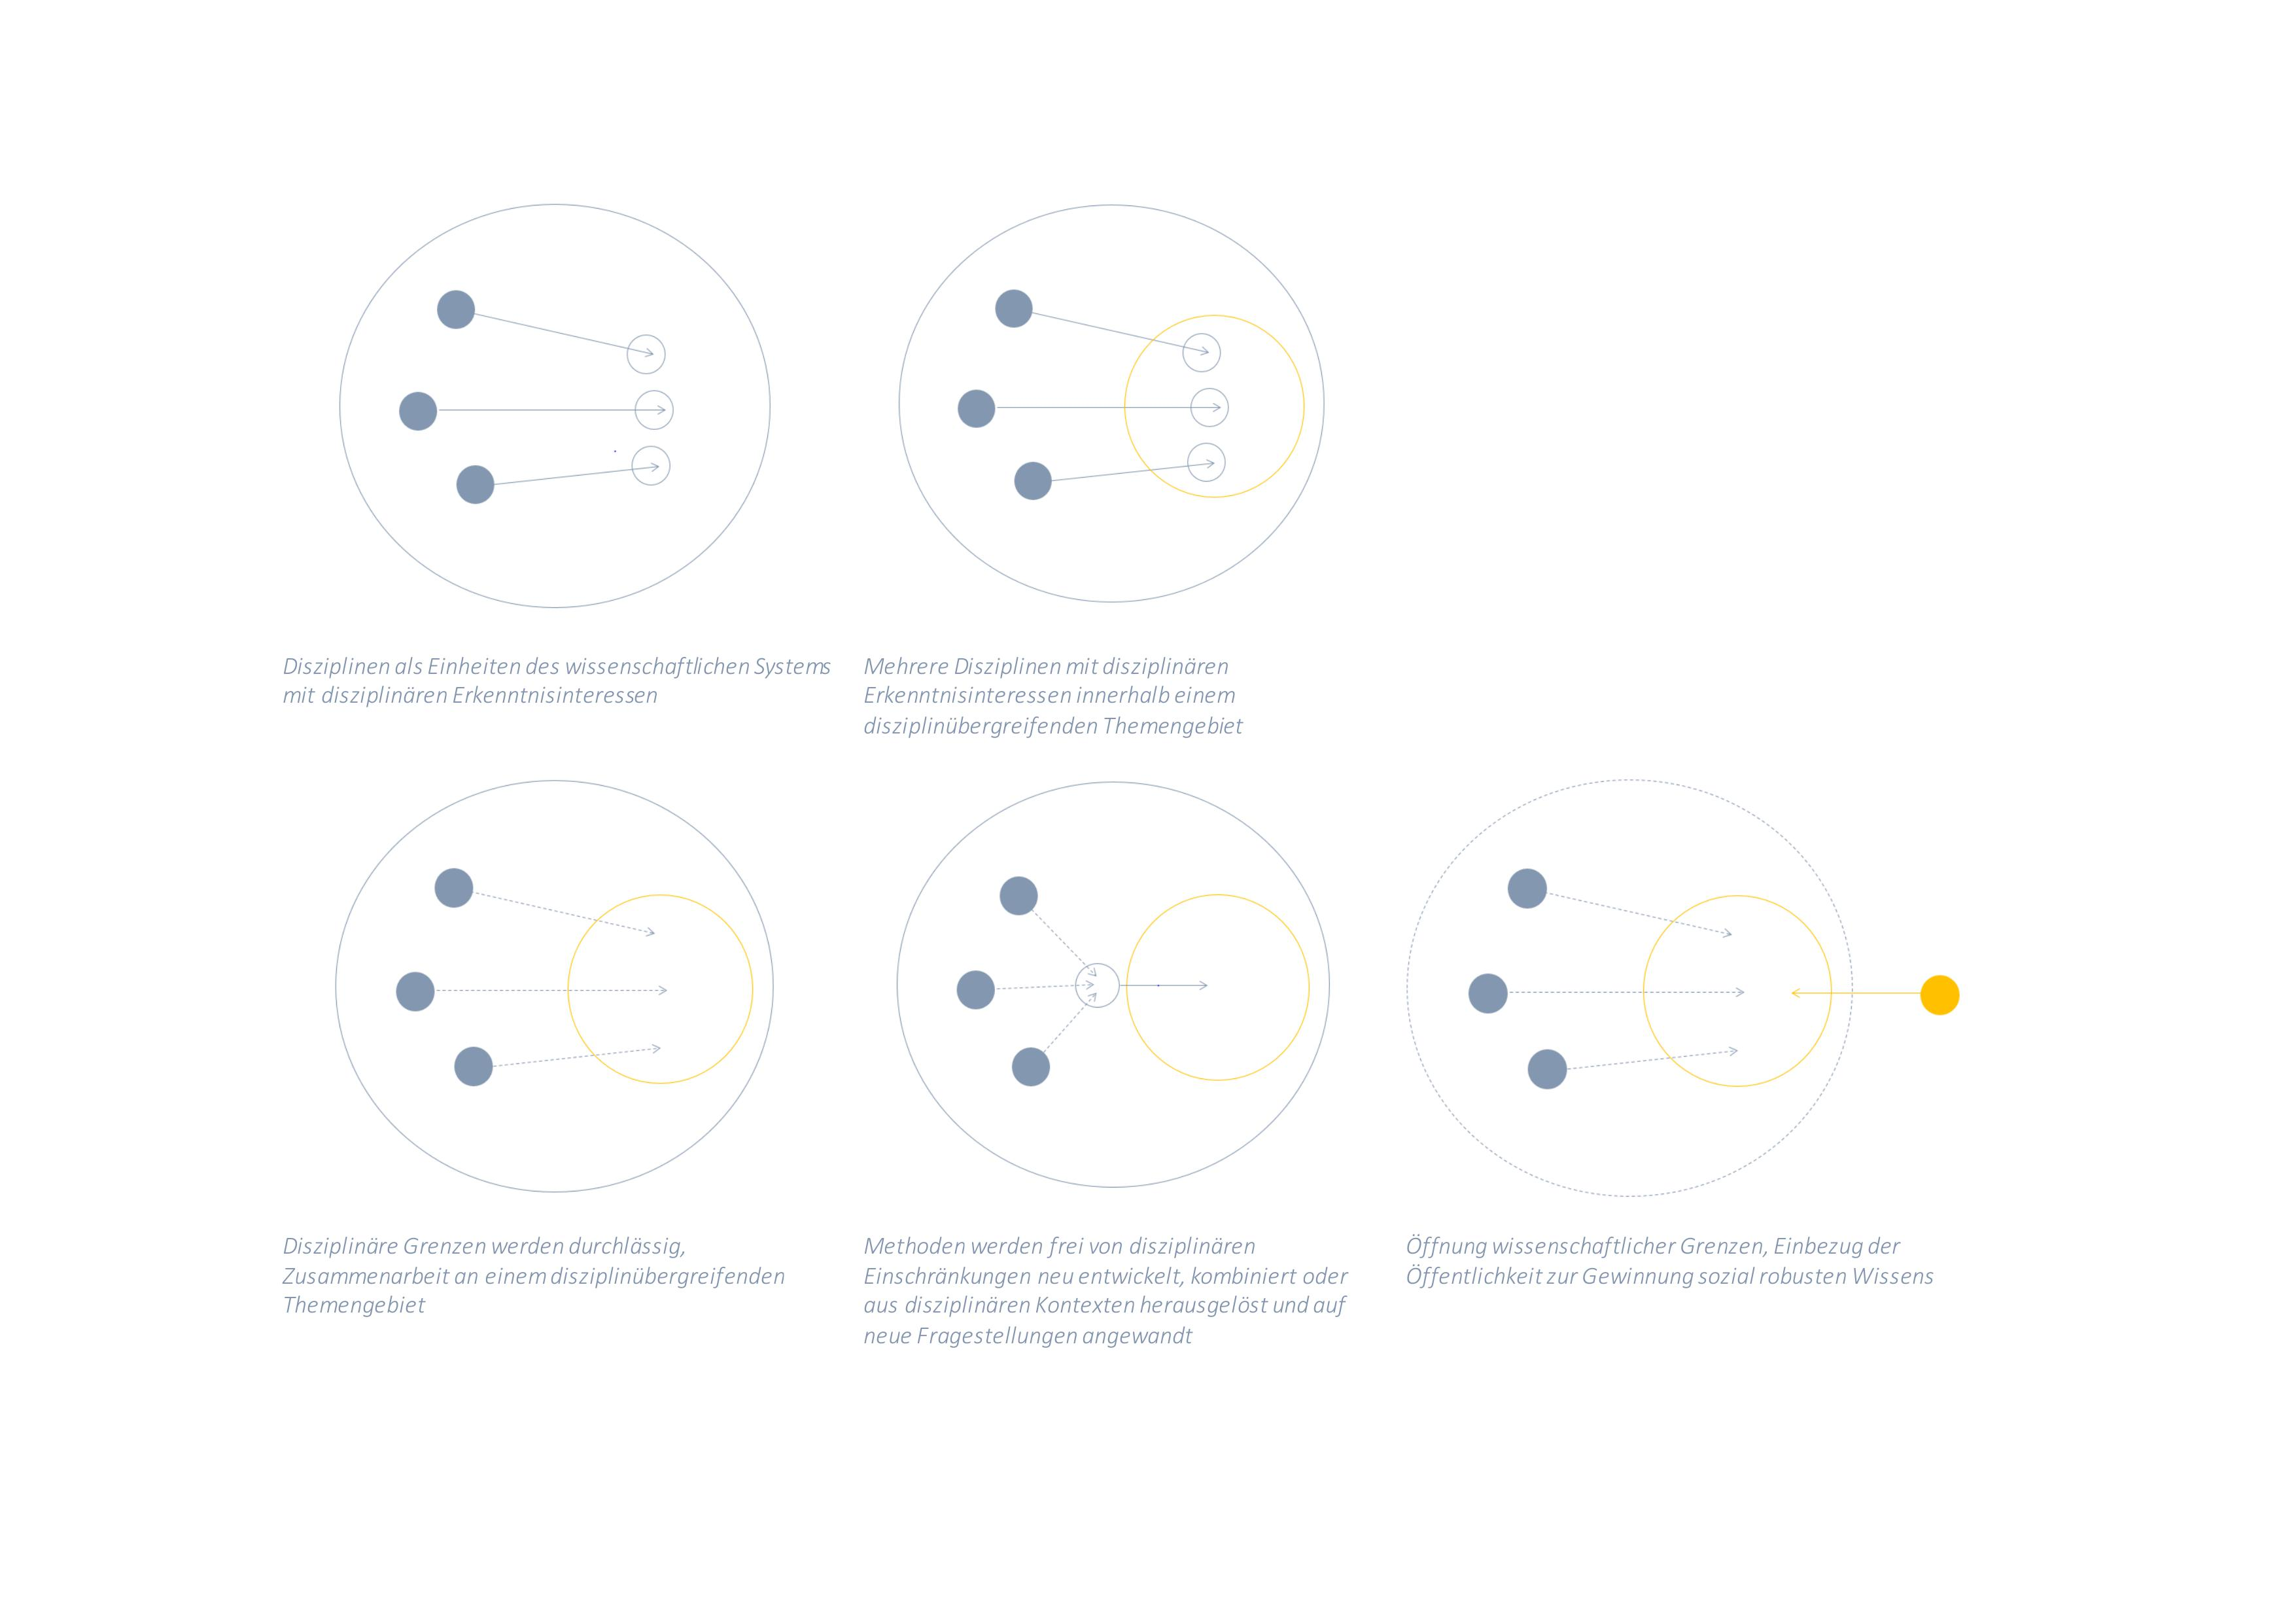
\includegraphics{img/Metamorphose_X.jpg}
\caption{Metamorphose der X-Disziplinarität}
\end{figure}

\section*{Verortung der
Informationswissenschaft}\label{verortung-der-informationswissenschaft}

Die disziplinäre Verortung der Informationswissenschaft steht im engen
Zusammenhang mit dem jeweiligen Verständnis ihres Hauptgegenstandes
\enquote{Information} und den, mit diesem einhergehenden, Elementen --
Daten, Wissen und im weiteren Sinne dem Dokument. Nahezu jede
wissenschaftliche Disziplin beschäftigt sich mit Information und
beansprucht ein eigenes, voneinander sehr unterschiedliches Verständnis
dieser. Information, das Nutzen und Nachdenken über diese, verändert
sich stetig und ist besonders aufgrund ihrer gesellschaftlichen
Bedeutung von politischen, rechtlichen und sozialen Entwicklungen
beeinflusst. In Hinblick auf eine Einordnung der
Informationswissenschaft ist es wichtig, eine Beschreibung von
Information vorzunehmen, die zeitlich und disziplinär lokal ist.

Lange Zeit bezog man sich innerhalb der Informationswissenschaft auf das
Sender-Empfänger-Modell von Claude Shannon und Warren Weaver; dieses
geriet jedoch aufgrund seines rein statistisch-mathematischen
Verständnisses von Information in die Kritik. Im deutschsprachige Raum
sind aktuell die Definitionsversuche Rainer Kuhlens maßgebend. Dieser
beschreibt, dass Information ihren Ausgang von Wissen nimmt und Wissen
somit den Grundstoff zur Entstehung von Informationen darstellt. Kuhlen
spricht von einem doppelten Transformationsprozess: Transformation 1:
Durch einen Prozess der Informationserarbeitung transformiert sich
potentiell relevantes Wissen in Information. Transformation 2:
Information wird durch den Prozess des zu potentiell relevantem Wissen.
(vgl. Kuhlen 2013, S. 4) Es kommt aufgrund des Informationsprozesses zur
Veränderung der Wissensstruktur.

\begin{figure}
\centering
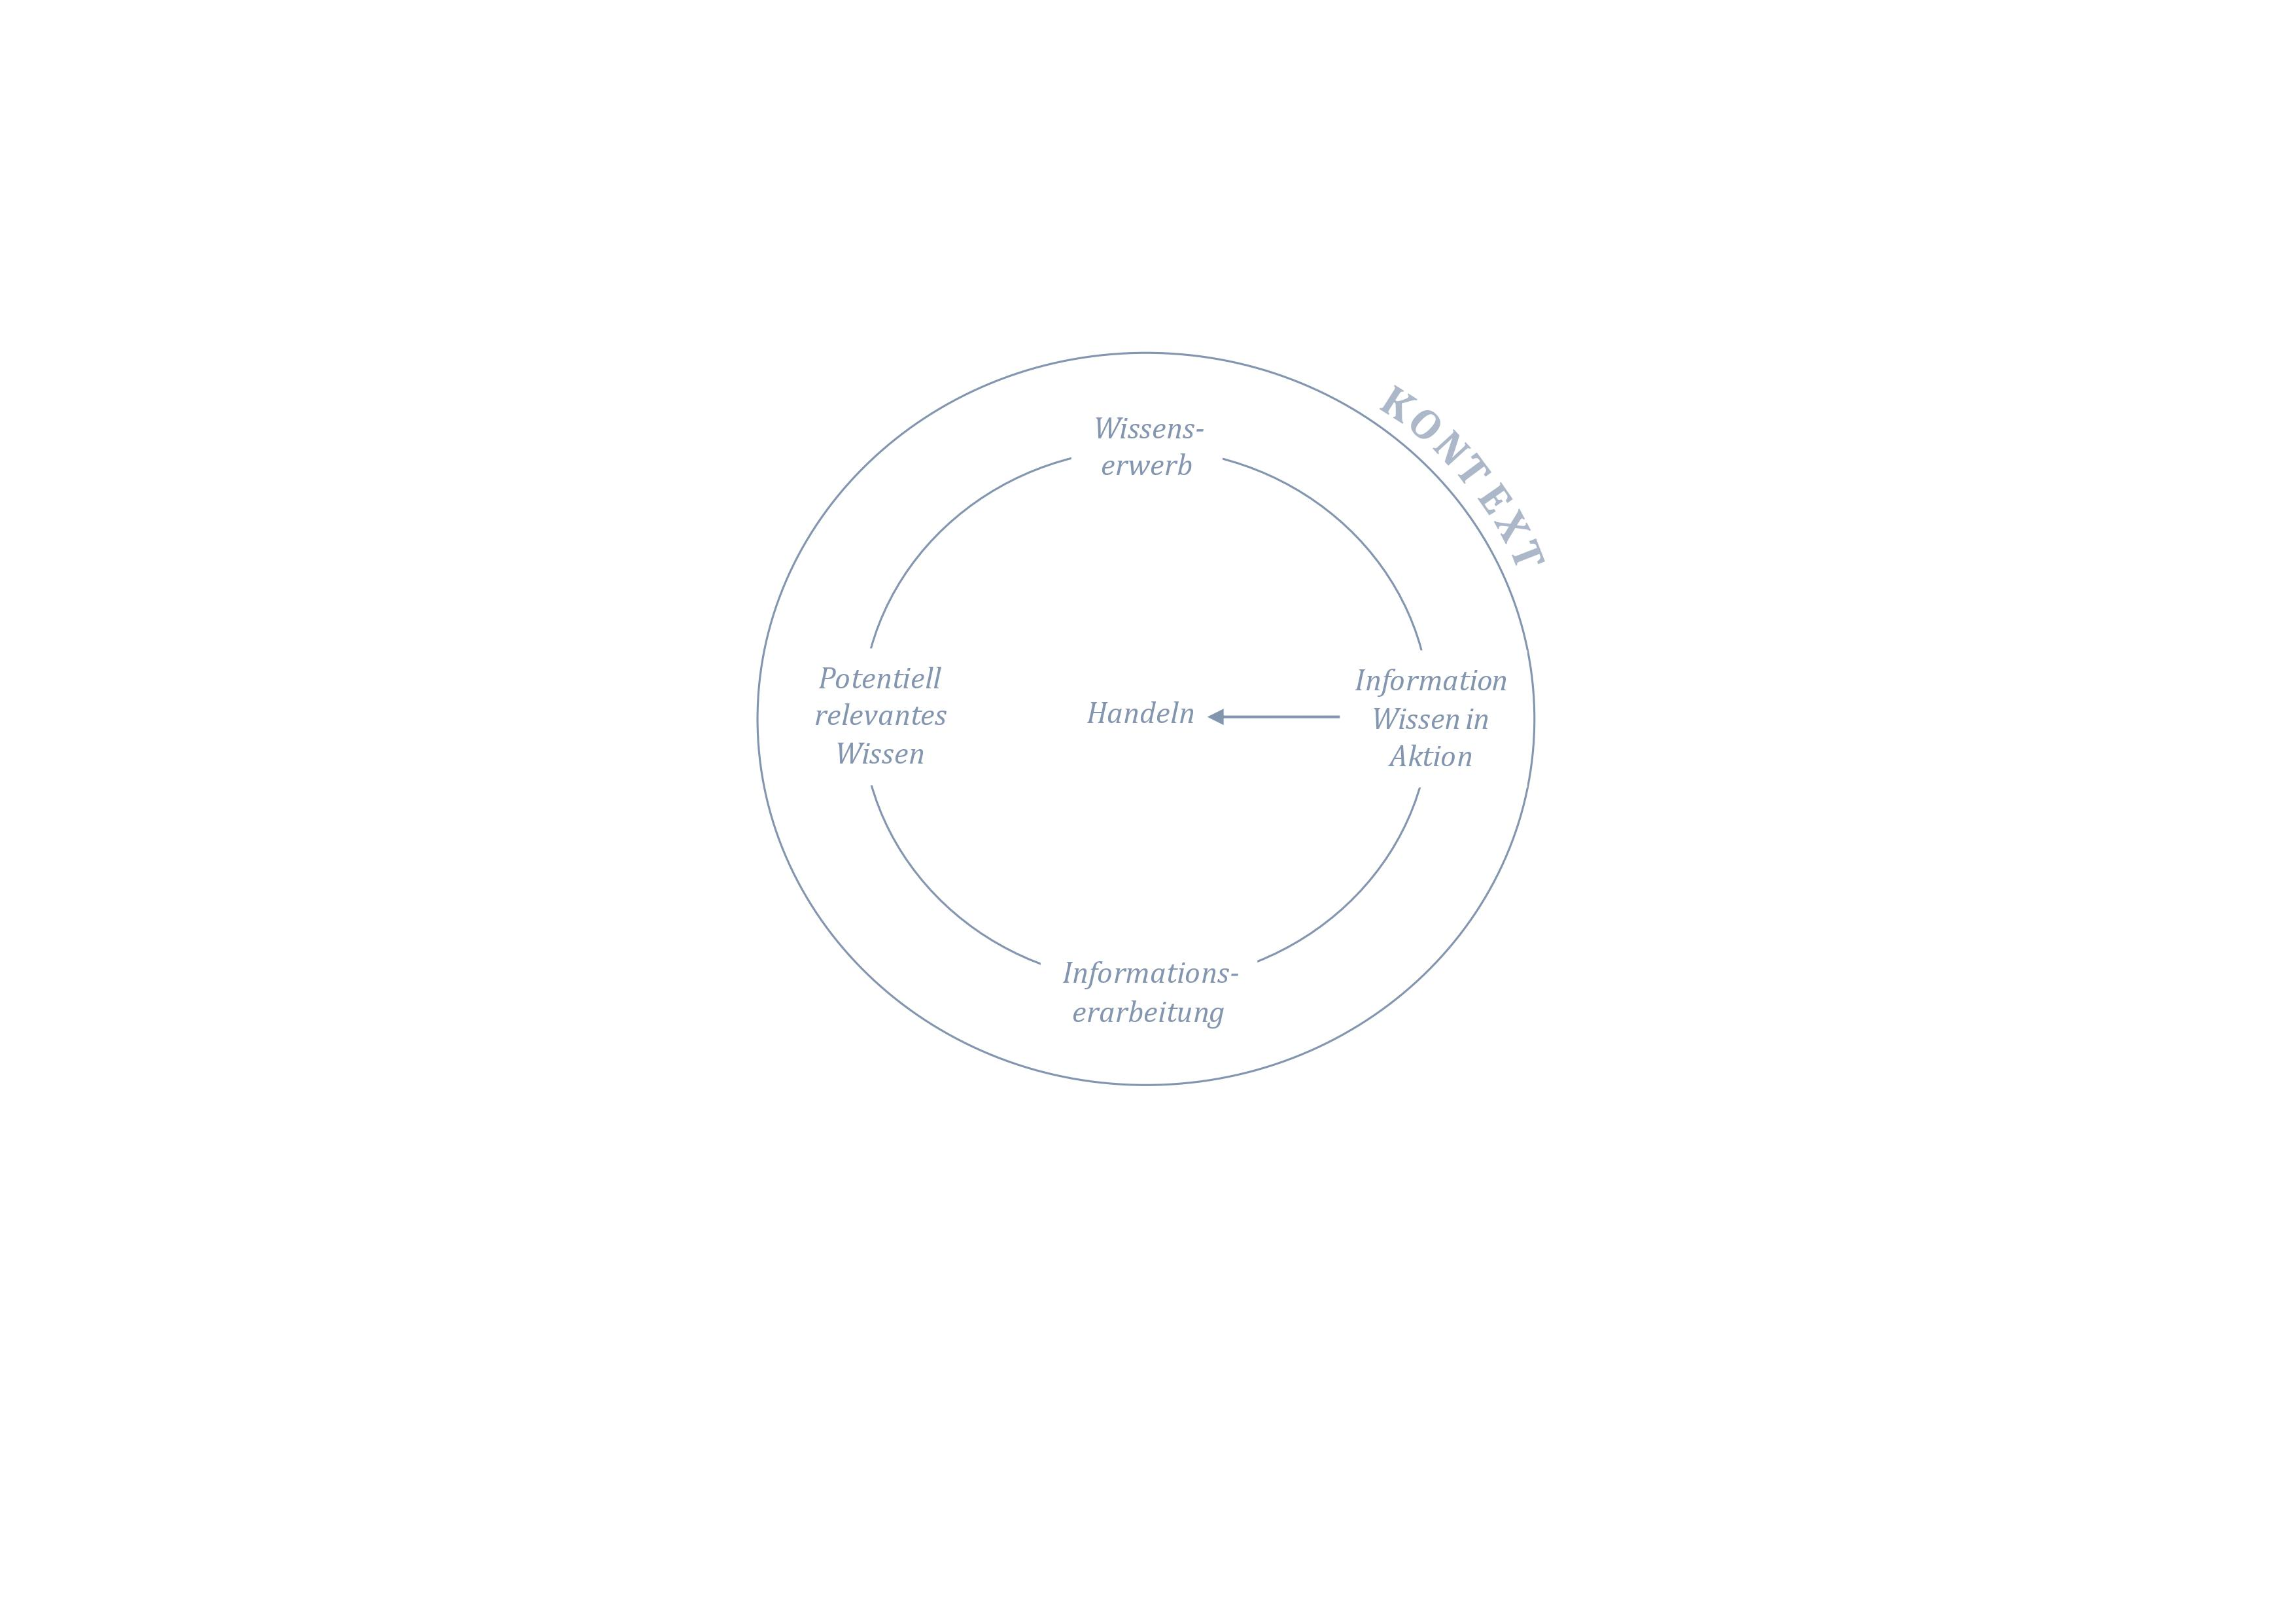
\includegraphics{img/Transformation_Information.jpg}
\caption{Transformationsprozess von Information und Wissen nach Kuhlen}
\end{figure}

Wissen kann als \emph{\enquote{Bündel von Aussagen über materielle oder
immaterielle Objektbereiche}} verstanden werden, welches
\emph{\enquote{verfügbar {[}ist{]} sobald es in irgendeiner medialen
Form repräsentiert ist.}} (Kuhlen 2013, S. 2) Die mediale Form
beschreibt nicht zwingend ein sprachlich oder schriftlich fixiertes
Dokument, sondern vielmehr das \enquote{kognitive Objekt} ein
\enquote{immaterielles Substrat}. Information stellt eine
\emph{\enquote{{[}\ldots{}{]} subjektive Rezeption von repräsentiertem
Wissen {[}\ldots{}{]}}} (Ebd. 2013, S. 2) dar -- eine vom Kontext des
Rezipienten abhängige Interpretation. Diese Information gilt erst als
solche, sobald sie für den Rezipienten von Nutzen und somit
handlungsrelevant ist. Anstelle eines hierarchischen Modells, wie
beispielsweise in der DIKW-Hierarchie nach Russell L. Ackoff, vertritt
Kuhlen eine funktionale Unterscheidung zwischen formalsyntaktischen,
semantischen und pragmatischen Ebenen von Information.

Parallelen zu Kuhlens Theorie sind beispielsweise in Michael Bucklands
dreiteiliger Informations-Definition zu erkennen. Buckland unterteilt
in: {[}1{]} \emph{Information-as-knowledge} -- erlangtes Wissen, dieses
wurde dadurch erlangt, informiert worden zu sein {[}2{]}
\emph{Information-as-process} -- über etwas informiert werden {[}3{]}
\emph{Information-as-thing} -- das physische Dokument.

Die erste Ebene ähnelt Kuhlens Transformationsprozess 2: Information
wird durch Wissenserwerb (den Prozess informiert worden zu sein) zu
potentiell relevanten Wissen. Die zweite Ebene gleicht dem
Transformationsprozess 1: in diesem entsteht durch den Erhalt relevanter
Information im Prozess (aus Wissen) Information. Auch Buckland sieht
Informationen als situationsgebunden und damit handlungsrelevant. Wissen
und Information bilden \emph{\enquote{intangible}} -- unfassbare --
Einheiten. Die dritte Ebene widmet sich deshalb explizit der physischen
Repräsentation von Wissen, in Form von Dokumenten.

Kuhlen leitet aus den dargestellten Überlegungen die Definition
\emph{\enquote{Information ist Wissen in Aktion und Kontext}} (Kuhlen
2013, S. 2) ab und hebt besonders die Handlungsrelevanz hervor. Die
ursprüngliche Definition bezog sich lediglich auf \emph{\enquote{Wissen
in Aktion}} und blendete vorerst den Kontext aus. Deutlich wird eine
einschlägige Veränderung des Verständnisses des Hauptgegenstandes und
damit einhergehend eine Veränderung des Verständnisses der Disziplin als
Ganzes. Besondere Bedeutung hat für die Informationswissenschaft, der
Definition von Kuhlen zufolge, der Aspekt der Handlungsrelevanz und
damit einhergehend die Nutzung und Nutzbarmachung von Informationen. Die
Abwendung vom technischen hin zum eher pragmatischen Informationsbegriff
ist in der Entwicklung der Informationswissenschaft deutlich
nachzuvollziehen.

\subsection*{Die paradigmatische Entwicklung der
Informationswissenschaft}\label{die-paradigmatische-entwicklung-der-informationswissenschaft}

Disziplinen sind \emph{\enquote{{[}..{]} nichts Naturgegebenes, sondern
etwas durch die Wissenschaftsgeschichte Gegebenes.}} (Mittelstraß, 1987,
S. 153) Ihre Grenzen, wie Mittelstraß mit diesem Satz aussagen will,
sind historische und nicht nur theoretische. Auch die
Informationswissenschaft ist -- wie jede wissenschaftliche Einheit --
historisch gewachsen.

Thomas S. Kuhn prägte den Begriff des Paradigmas. Dieses beschreibt
bestimmte Entwicklungen innerhalb der wissenschaftlichen Praxis, welche
die aktuelle Forschung formen und leiten. Nach Kuhn wird die Entstehung
und Veränderung einer Disziplin durch wissenschaftliche Revolutionen
ausgelöst. Innerhalb einer wissenschaftlichen Revolution stehen sich
zwei oder mehrere Paradigmen, in Form von Theorien, gegenüber. Häufig
stellt sich die alte Theorie als Grenzfall der Neuen heraus und es kommt
zu einer \emph{\enquote{{[}\ldots{}{]} Verschiebung des Begriffsnetzes
{[}\ldots{}{]}, durch welches die Wissenschaftler die Welt betrachten.}}
(Kuhn 1976, S. 115) -- eine kollektive Wahrnehmungsverschiebung. (vgl.
Kuhn 1976) Paradigmatisch lassen sich für die Informationswissenschaft
vier Hauptphasen bestimmen (vgl. Capurro 2001; Kuhlen 2013; Bawden,
Robinson 2012):

{[}1{]} Klassifikations-Paradigma

Ende des 19. Jahrhunderts kam es aufgrund des wissenschaftlichen
Fortschritts zu einer rapiden Zunahme wissenschaftlichen Wissens,
ausgelöst unter anderem durch starke Publikationszuwächse. Eine Ordnung
und Strukturierung der vorliegenden Wissensbestände wurde dringend
erforderlich. So entstanden in dieser Phase erste, universell angelegte
Klassifikations- und Bibliothekssysteme mit dem Ziel der Optimierung
beziehungsweise Nutzbarmachung von (wissenschaftlichem) Wissen.
Allgemein ist die erste Phase durch eine
bibliographisch-dokumentarische, klassifikatorische Sicht auf
Information und Wissen charakterisiert. Sie kennzeichnet grundlegende
Begriffe informationswissenschaftlicher Tätigkeiten: Auswerten,
Bereitstellen, Suchen und Finden, Organisieren und Präsentieren von
Information und Wissen. (vgl. Kuhlen 2013, S. 12ff.)

{[}2{]} Retrival-Paradigma

Die zweite Phase kennzeichnet eine Abwendung von der rein
bibliographischen hin zur inhaltlichen Erschließung. Ein stark prägendes
Ereignis war der Sputnik-Schock (1957) und die, mit diesem
einhergehenden, Förderprogramme, welche wissenschaftlichen Fortschritt,
Innovation und damit Wissenszuwachs vorantreiben sollten. Wie zuvor in
der ersten Phase wurde die Rückständigkeit wissenschaftlicher
Klassifikationssysteme und die fehlende Zugänglichkeit der zunehmenden
Wissensbestände sichtbar. Beeinflusst durch den Weinbergreport (1963)
kam es infolgedessen zu einer Intensivierung der Informationsarbeit und
Ausweitung der Informationsinfrastruktur. Entwicklungen erster
Online-Datenbanken sowie automatischer Indexierungsverfahren konnten
aufgrund fortschreitender Computertechnik realisiert werden. Die
Informationsarbeit gewann zunehmend an Bedeutung -- es kam zur
Institutionalisierung der Informationswissenschaft. (vgl. Stock, Stock
2012, S. 402f.) Das bibliographische Verständnis wandelt sich in der
zweiten Phase, durch die Automatisierung der Informationsarbeit, hin zu
einem mathematisch-technischen. (vgl. Kuhlen 2013, S. 12ff.)

{[}3{]} Kognitives Paradigma

Die dritte Phase begann in den 1980er Jahren. Ausschlaggebend für den
Umbruch waren neue Forschungen der kognitiven Psychologie und der
künstlichen Intelligenz, welche behaupteten, menschliche
Informationsverarbeitung durch Computer nachbilden zu können. Diese
eingeschränkte Betrachtung menschlichen Informationsverhaltens wurde von
Vertreter\_innen der Informationswissenschaft stark kritisiert. Die
menschliche Informationsverarbeitung, so die Kritik, sei viel komplexer
als sie zu diesem Zeitpunkt von Computern dargestellt werden könnte. Die
Informationswissenschaft stellte, daraus resultierend, neben der
technischen Komponente den Menschen (als kognitives Subjekt) in den
Mittelpunkt ihrer Forschung. In dieser Phase entwickelte sich eine
systemorientierte, technische Sicht auf Information, welche durch eine
kognitive Sicht Ergänzung fand. (vgl. Kuhlen 2013, S. 12ff.)

{[}4{]} Praxis-Paradigma

Ende des 20. Jahrhunderts kam es infolge übergreifender Vernetzung,
durch technische Kommunikationssysteme und die Verbreitung des
Internets, zu einer schrittweisen Öffnung vorliegender Informations- und
Wissensbestände in allen Bereichen der Gesellschaft. In der sich
entwickelnden Informations- und Wissensgesellschaft werden Fragen nach
Offenheit, Freiraum sowie Recht auf Nutzung und Verbreitung von
Information notwendig und stellen einen bedeutenden Themenbereich
informationswissenschaftlicher Diskussionen dar. Die
Informationswissenschaft entwickelt sich damit wieder zunehmend zu einer
sozial-, geisteswissenschaftlich ausgerichteten Disziplin -- der Mensch
und sein Informationsbedürfnis rücken vermehrt in den Mittelpunkt. Zudem
orientiert sich die Forschungstätigkeit der Informationswissenschaft, in
theoretischer Hinsicht, an situativen und sozialen Praxisgegebenheiten
und damit an dem direkten Gebrauch von Informationen. (vgl. Kuhlen 2013,
S. 13)

\begin{figure}
\centering
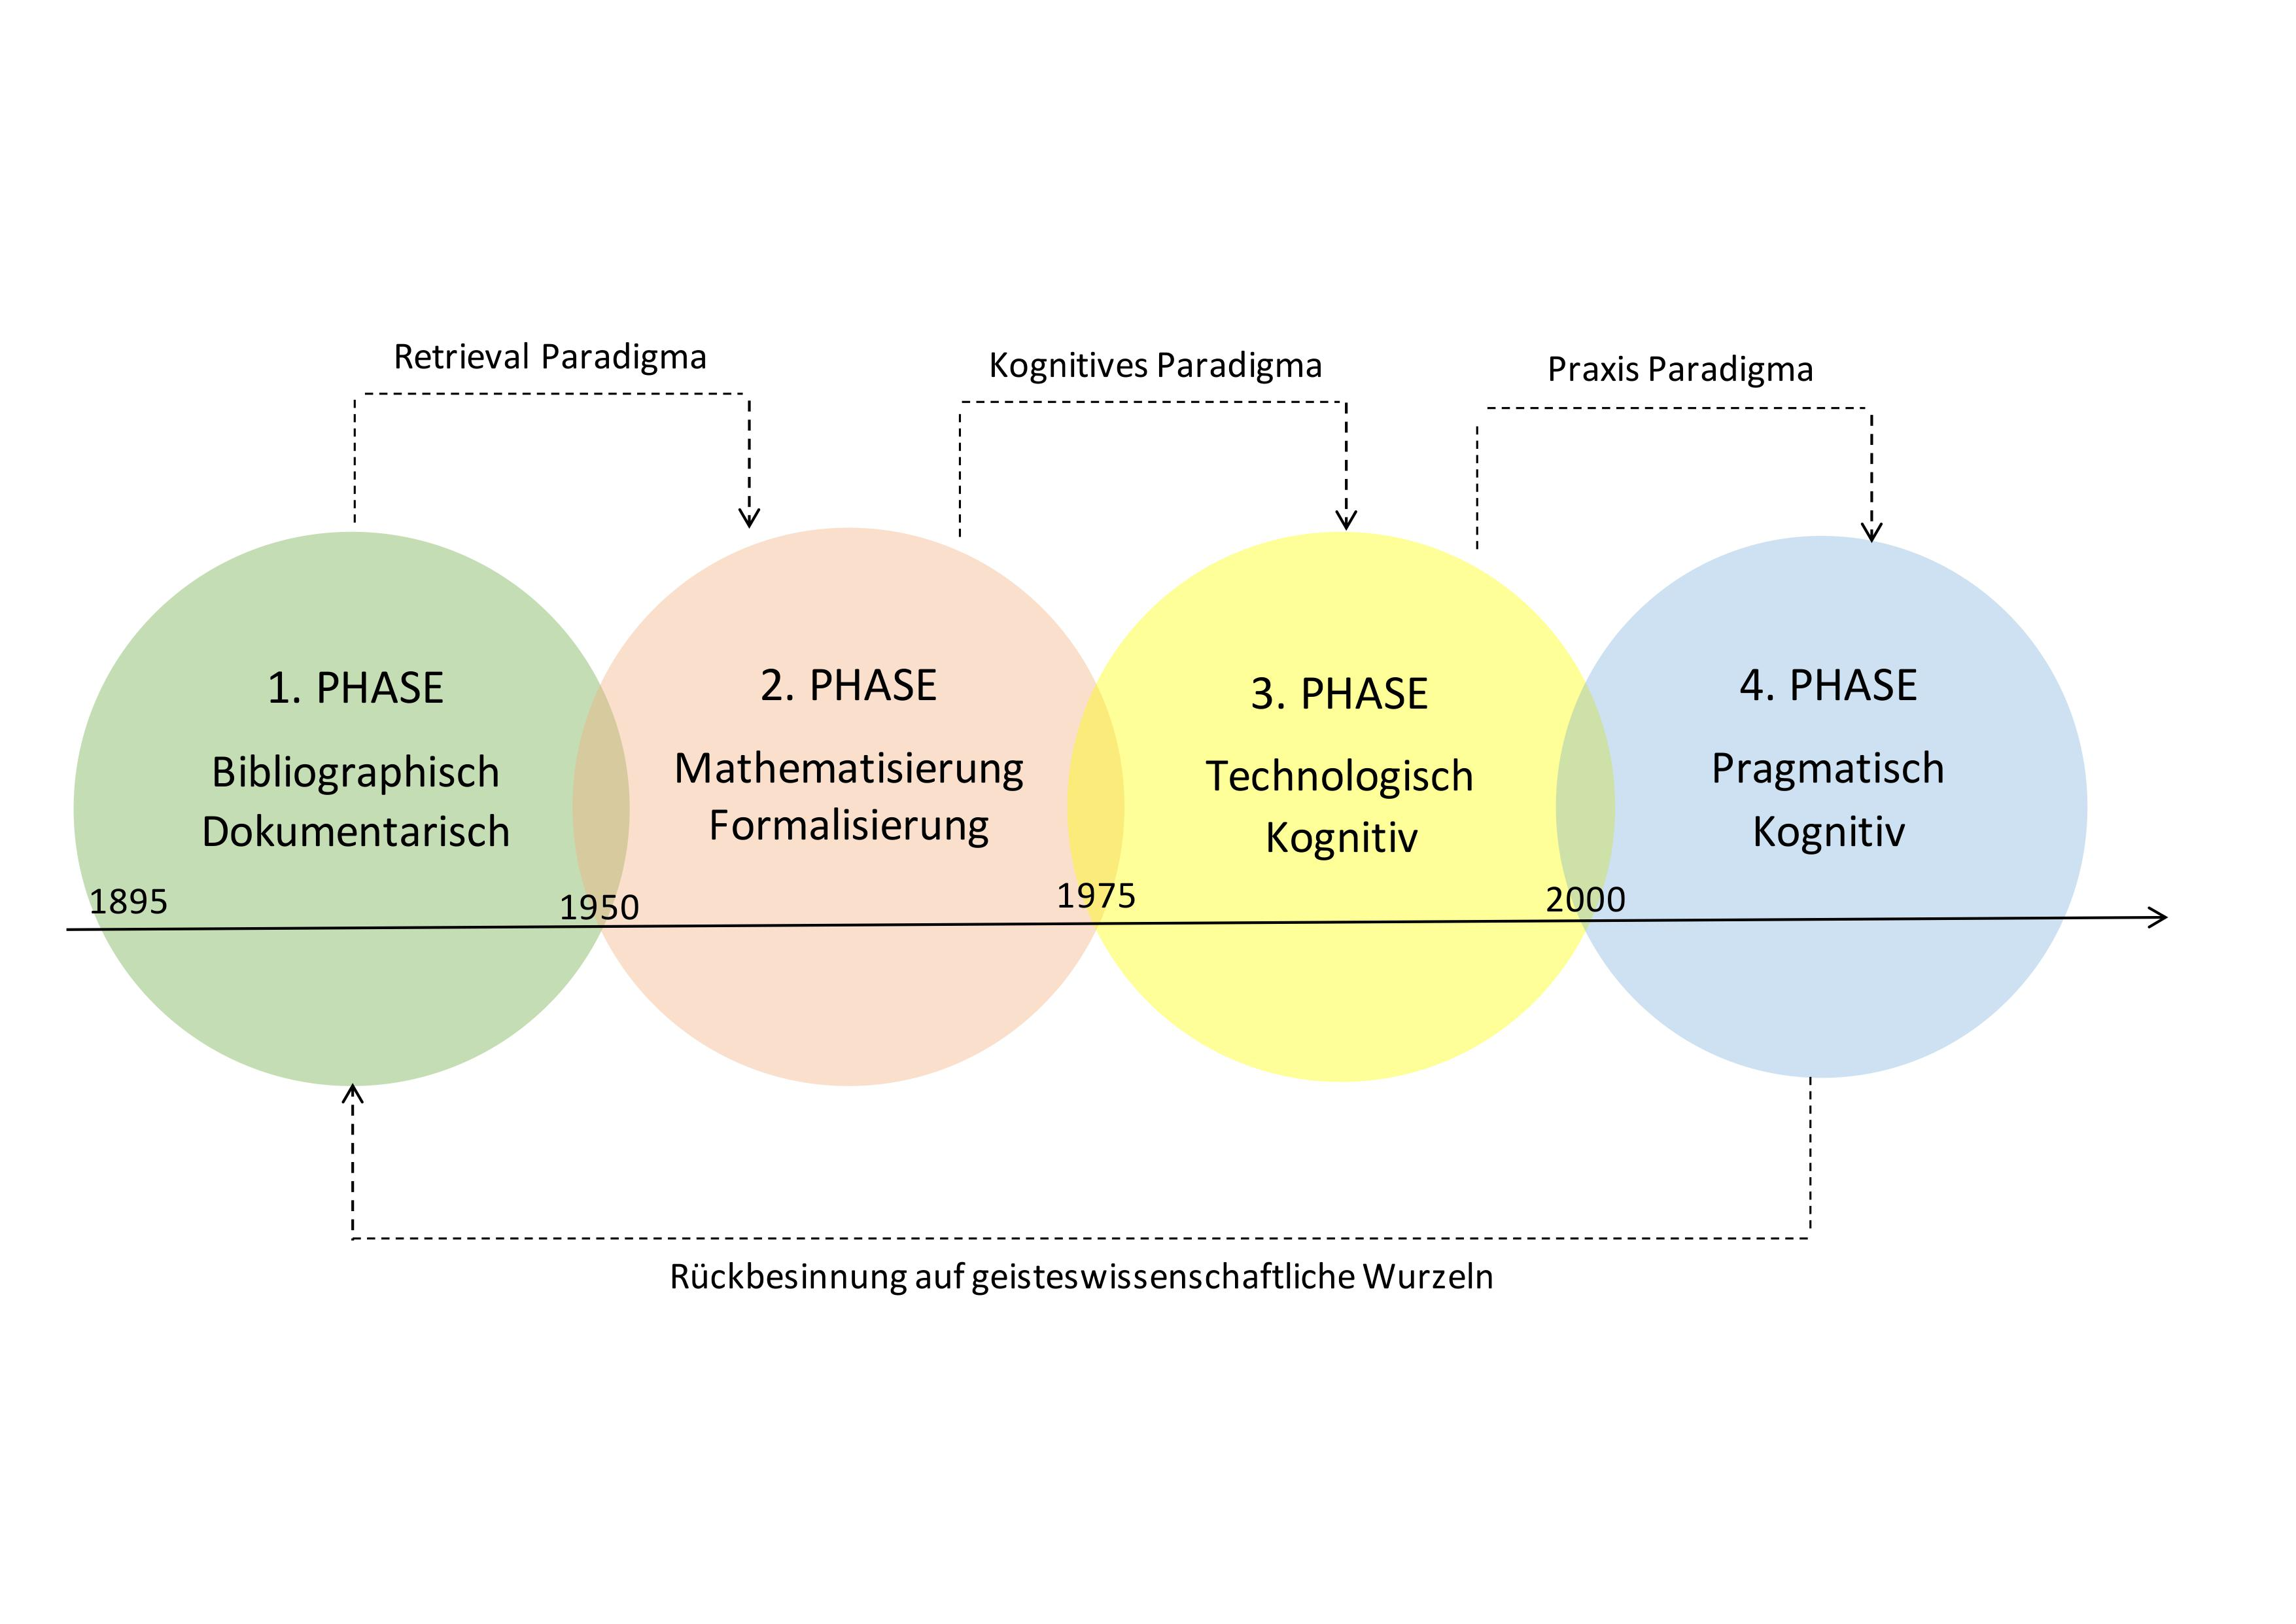
\includegraphics{img/Phasen_IW.jpg}
\caption{Vier-Phasen Entwicklung der Informationswissenschaft}
\end{figure}

Die Informationswissenschaft entwickelte sich, wie auch am aktuellen
Verständnis von Information deutlich geworden ist, von der anfänglich
bibliographisch, zwischenzeitlich mathematisch-technisch stark
beeinflussten, hin zu einer pragmatisch-kognitiven Disziplin. Die
technische Seite, die mit den aktuellen Entwicklungen in direktem
Verhältnis steht, darf in dieser Betrachtung jedoch nicht außer Acht
gelassen werden: Informationswissenschaft als Geistes- und
Sozialwissenschaft mit Blick auf (und direkter Beeinflussung durch)
aktuelle technische Entwicklungen. Kuhlen plädiert deshalb, in
Verbindung mit der aktuellen Verortung der Informationswissenschaft, für
eine Kombination der dritten und vierten Phase. (vgl. Kuhlen 2013, S.
12ff.) Und auch Rafael Capurro weist darauf hin, dass sich die
Informationswissenschaft in ihrer Tätigkeit auf die gesellschaftlichen
Fragen konzentrieren sollte. Die technischen Aspekte sollten zwar
betrachtet, aber nicht als Hauptaufgabe der Forschung angesehen werden,
sonst würde sich die Informationswissenschaft, so Capurro, nicht von der
Informatik unterscheiden. (vgl. Treude, 2001)

\subsection*{X-Disziplinarität der
Informationswissenschaft}\label{x-disziplinarituxe4t-der-informationswissenschaft}

Es wurde zuvor festgestellt, dass sich die Informationswissenschaft mit
\enquote{Informationen} auseinandersetzt; dabei begrenzt sie sich auf
ausgewählte Ebenen des Begriffs: Sie vertritt, ein pragmatisches
Verständnis von Information und widmet sich, aus dieser
handlungsrelevanten Sicht heraus, konkret der Nutzung und Nutzbarmachung
von Informationen. Um dem Begriff der Information gerecht zu werden,
erfordert es darüber hinaus x-disziplinärer Kooperation.

In zahlreichen Diskussionen wird demzufolge auf die X-Disziplinarität
der Informationswissenschaften hingewiesen -- eine einheitliche Meinung
darüber, welche Disziplinaritätenart die Informationswissenschaften
verkörpert oder was sie zu einer grenzüberschreitenden Wissenschaft
macht, existiert nicht. Im Folgenden wird, auf der Grundlage der
Konzept-Definitionen, der x-disziplinäre Fachdiskurs innerhalb der
Informationswissenschaft untersucht und dargestellt. Es folgt eine
Auswertung einschlägiger informationswissenschaftlicher Publikationen
mittels Gegenüberstellung und diskursiver Einordnung der
themenspezifischen (impliziten sowie expliziten) Stellungnahmen. Um die
inhaltliche Bandbreite des Diskurses zu erfassen, sind die Aussagen in
drei Hauptthemen unterteilt: wissenschaftshistorische,
wissenschaftssoziologische und außerwissenschaftliche Begründungen.

\textbf{Wissenschaftshistorische Begründungen}

Die Bedingungen aus denen die Informationswissenschaft entstand wurden
bereits 1968 von Harold Borko als Grund für ihre Interdisziplinarität
beschrieben: \emph{\enquote{{[}\ldots{}{]} it is an interdisciplinary
science derived from and related to such fields as mathematics, logic,
linguistics, psychology {[}\ldots{}{]}.}} (Borko, 1968, S. 1) Begründet
wird die Interdisziplinarität unter anderem durch die Entstehung aus und
der sich daraus ergebenden Verbindungen zu anderen Disziplinen. Borko
bezieht sich auf die erste Phase der Entstehung der
Informationswissenschaft, in welcher die Zugänglichmachung von
Informationen für die Wissenschaft im Vordergrund standen: Die
Informationswissenschaft stand nach dieser Auslegung als
Informationsvermittlerin zwischen den Disziplinen -- als
\enquote{Inter}-Disziplin im angewandten, nicht im theoretischen Sinne.

Die Einordnung Borkos führte seitdem zur wiederholten Betitelungen der
Informationswissenschaft als \enquote{von Natur aus interdisziplinär}.
Buckland et al. wiesen kürzlich darauf hin, dass diese Aussage in
aktuellen Diskussionen von den meisten Vertreter\_innen als gegeben
angesehen und ohne selbige zu hinterfragen, übernommen wird. (vgl.
Arafat et al. 2014, S. 1) In den 1960er Jahren hatte die
Interdisziplinarität ihren Höhepunkt innerhalb
wissenschaftstheoretischer und -politischer Diskussionen und fand auch
in der Informationswissenschaft als \emph{\enquote{{[}\ldots{}{]}
euphorisches Schlagwort einer wissenschaftskritischen Einstellung
{[}\ldots{}{]}}} (Ryser 2016) seine Verwendung.

Neben der Interdisziplinarität finden, in Hinblick auf die
wissenschaftshistorischen Begründungen, weitere x-disziplinäre Konzepte
Verwendung. Bawden und Robinson beispielweise stellen die
Informationswissenschaft mit dem Begriff der \enquote{Metadisziplin}
über die Disziplinen und vergleichen sie in diesem Zusammenhang mit der
Philosophie. Philosophie, als Metawissenschaft betrachtet, hinterfragt
das von der Wissenschaft hervorgebrachte Wissen, weshalb sich für jede
wissenschaftliche Disziplin Anknüpfungspunkte an philosophische
Erkenntnisse ergeben. Sie begründen ihre Aussage wie folgt:
\emph{\enquote{{[}Information Science has{]} links with all other
disciplines, since all have some information and knowledge extensions,
and hence information scientists may contribute to all.}} (Bawden,
Robinson 2013, S. 6) Bawden und Robinson nehmen damit direkt Bezug auf
Marcia J. Bates` Modell der Meta-Disziplinen, welches die
Informationswissenschaft als \enquote{orthogonal} beschreibt:
*\enquote{The}orthogonal" disciplines, or, \enquote{meta-disciplines,}
shape the subject matter of all the traditional disciplines according to
the social purpose of the meta-discipline {[}\ldots{}{]}.``* (Bates
2007) Der Begriff Meta-Disziplin wird hier, ähnlich dem
transdisziplinären Konzept von Stichweh, ausgelegt als: Eine Disziplin,
die über allen Disziplinen steht und die Funktion einer
\emph{\enquote{disziplinübergreifende Ressourcen}} einnimmt. Nach diesem
Prinzip ist die Informationswissenschaft eine übergreifende Instanz,
welche als Grundlage für diverse Disziplinen dient; Verbindungsglied:
die Information.

Werner Kunz und Horst Rittel distanzierten sich bereits 1972 deutlich
von der Bezeichnung Metawissenschaft: \emph{\enquote{Die
Informationswissenschaften sind keine Metawissenschaften {[}\ldots{}{]}.
Sie erheben nicht den Anspruch, über den Wissenschaften zu stehen.}}
(Kunz, Rittel 1972, S. 12) Sie plädieren stattdessen für die Bezeichnung
transdisziplinär: ``*Sie sind gewissermaßen ‚quer` zu den
Objektbereichen der Disziplinen orientiert, weshalb man sie auch als
transdisziplinär bezeichnet.``* (Ebd. 1972, S. 12) Auch in aktuellen
Theorien ist wieder eine Zunahme des Begriffs Transdisziplinarität zu
erkennen, so gewinnt sie als
\emph{\enquote{wissenschaftspolitisch{[}es{]} neues Schlagwort}} (Hobohm
2015, S.5) an Zuspruch. Die Informationswissenschaft versucht,
\emph{\enquote{da mit einer Selbstzuschreibung als Interdisziplin
mittlerweile die akademischen Pfründe verloren gehen {[}sic{]}
{[}\ldots{}{]}}} (Ebd. 2015, S. 5), sich, aus der Not heraus, als
Transdisziplin zu etablieren.

Hans-Christoph Hobohm beschreibt die Transdisziplinarität in diesem
Zusammenhang nicht als \enquote{quer} zu den Disziplinen, sondern,
ähnlich der Definition von Mittelstraß, als eine Zusammenarbeit die
``*dort {[}\ldots{}{]} notwendig {[}wird{]}, wo i. w. S. globale
Probleme zu einer Art übergreifenden Fachlichkeit führen
{[}\ldots{}{]}``* (Ebd. 2015, S. 5) Dieser disziplinübergreifende
Zusammenschluss generiert über einen nicht genau zu definierenden
Zeitraum eine Transdisziplin. \emph{\enquote{Im Falle der
Informationswissenschaften (im Plural) {[}\ldots{}{]}}} so Hobohm
\emph{\enquote{{[}\ldots{}{]} wage ich zu behaupten, dass wir hierzu
gerade dabei sind am eigenen Leib, dieses Phänomen zu beobachten.}}
(Ebd. 2015, S. 5) Die sich auflösenden Disziplinen sind in diesem Fall
die Bibliotheks-, Dokumentations- und Archivwissenschaft. In Frage steht
jedoch, ob es sich bei diesen um eigenständige Disziplinen oder um
Anwendungsfelder der Informationswissenschaft handelt:
\emph{\enquote{One area of debate has been the relation with
\enquote{adjacent} disciplines such as librarianship, archiving,
information systems and computer science; views here have ranged from
such disciplines being the same thing, entirely distinct, distinct but
interdependent, distinct but naturally linked and part of a composite
discipline.}} (Robinson, Karamuftuoglu 2010) So werden die Disziplinen
auch bei Hobohm mal als Grund-, mal als Subdisziplinen bezeichnet. Als
wissenschaftliche Subdisziplinen müssten sich diese zu irgendeiner Zeit
von der Informationswissenschaft abgespalten haben und wären dieser in
der hierarchischen Ordnung des wissenschaftlichen Systems untergeordnet.
Die \emph{\enquote{übergreifende Fachlichkeit}} würde eine
Entdifferenzierung -- die Wiederherstellung der ursprünglichen
Disziplinarität -- beschreiben, was wiederum dem Ursprungsgedanken
x-disziplinärer Konzepte -- der Wiederherstellung der
\emph{\enquote{Einheit der Wissenschaft}} -- entspräche.

Hjørland beschreibt X-Disziplinarität, dieser Idee folgend, als einen
Prozess, welcher mit der Multidisziplinarität beginnt und sich am Ende,
als Ergebnis einer transdisziplinären Kooperation, als eigene Disziplin
formiert: \emph{\enquote{{[}\ldots{}{]} {[}S{]}ocial fields are dynamic
and changing. LIS for example, can be viewed as a field that started as
a multidisciplinary field {[}\ldots{}{]} which is developing towards a
monodiscipline in is own right.}} (Hjørland 2014, S. 207) Im Unterschied
zu Hobohm hat die Informationswissenschaft in dieser Betrachtung bereits
die x-disziplinäre Entwicklung abgeschlossen und sich als Disziplin
etabliert. Somit bestand die Informationswissenschaft nicht als
eigenständiges Konzept, sondern entwickelte sich erst durch den
Zusammenschluss unterschiedlicher Disziplinen über die Zeit. Am Beispiel
der Kooperation von Informationswissenschaft und Linguistik beschreibt
unter anderem Volkmar Engerer einen solchen Zusammenschluss. Er
bezeichnet die Kooperation als inter- beziehungsweise transdisziplinär,
macht aber gleichzeitig deutlich, dass es sich um eine, von der
Informationswissenschaft ausgehende, einseitige Kooperation -- und damit
\enquote{Nicht-Kooperation} -- handelt. (vgl. Engerer 2012) So
beschreibt er die Linguistik unter der Überschrift \enquote{Das
transdisziplinäre Paradigma: die Einverleibung linguistischer Konzepte}
als \emph{\enquote{aktive Spenderdisziplin}} (Engerer, 2012, S. 81). Die
Erweiterung erfolgte damit nicht durch kooperativen Zusammenschluss oder
als, wie für die Interdisziplinarität kennzeichnend, temporäre
Erweiterung des eigenen disziplinären Horizonts durch Überschreitung der
Grenzen, bezogen auf ein spezifisches Problem und kennzeichnet damit
keine X-Disziplinarität.

\textbf{Wissenschaftssoziologische Begründungen}

Kommunikative Ebene:

Weitere Begründungen lassen sich auf der kommunikativen Ebene
festmachen; zu dieser zählen unter anderem Zeitschriftenartikel und
Sammelbände, welche zunehmend in Gemeinschaft verfasst und
veröffentlicht werden, das führt vielfach zu der Annahme x-disziplinärer
Kooperation -- nicht selten wird jede Form der Zusammenarbeit mit Multi-
oder Interdisziplinarität gleichgesetzt. Innerhalb der
Informationswissenschaft weist unter anderem Kuhlen auf eine
Multidisziplinarität des Publikationsverhaltens hin. Er bezieht sich auf
eine 2012 von Lavière et al. durchgeführte Studie, die einschlägige
englischsprachige Zeitschriften auswertet und auf zentrale
Themenbereiche untersucht. Kuhlen hebt -- neben der Diversität der
innerhalb der Zeitschriften behandelten Themenbereiche -- die steigende
Anzahl der Artikel von Informationswissenschaftler\_innen innerhalb der
Publikationen anderer Disziplinen, sowie die Veröffentlichungen von
Vertreter\_innen anderer Disziplinen innerhalb
informationswissenschaftlicher Publikationen hervor. (vgl. Kuhlen, 2013,
S. 11f.) Die Aussage der Multidisziplinarität steht unkommentiert im
Raum: Es ist nicht ersichtlich in welcher Weise und Intensität eine
Zusammenarbeit der unterschiedlichen Akteure erfolgte oder ob die
Artikel einen Mehrwert für die jeweils andere Disziplin hatten.
Multidisziplinarität beschreibt die Bearbeitung eines Themas zur Lösung
eines disziplinübergreifenden Problems unter eigenen disziplinären
Schwerpunkten mit anschließender Zusammenstellung der einzelnen
Ergebnisse -- es findet keine Grenzüberschreitung statt. Die Tatsache,
dass Wissenschaftler\_innen anderer Disziplinen in
informationswissenschaftlichen Publikationsorgangen unter übergreifenden
Themen publizieren, begründet, dieser Beschreibung zufolge, eine
Multidisziplinarität.

Kuhlen bezieht sich mit der Aussage jedoch nicht auf die eigentliche
Publikationstätigkeit. Stattdessen stellt er im weiteren Textverlauf
eine andere Begründung für die Diversität auf: \emph{\enquote{Die für
die Informationswissenschaft festzustellende Multidisziplinarität ist
{[}\ldots{}{]} sicherlich der Attraktivität der Disziplin, da sie einer
Vielzahl von WissenschaftlerInnen aus ursprünglich anderen Disziplinen
ein attraktives Betätigungsfeld bietet {[}\ldots{}{]}}.} (Kuhlen 2013,
S. 12) Entscheidender Faktor ist demnach die
\emph{\enquote{Attraktivität der Disziplin}} für Wissenschaftler\_innen
anderer Disziplinen und eine daraus resultierende Diversität von
informationswissenschaftlichen Publikationen. Es stellt sich somit die
Frage, ob sich Wissenschaftler\_innen innerhalb der
Informationswissenschaft als:

{[}1{]} primäre Vertreter\_innen ihrer Herkunftsdisziplin sehen oder ob
es

{[}2{]} Wissenschaftler\_innen aus ehemals anderen Disziplinen sind,
welche sich mittlerweile auf die Informationswissenschaft spezialisiert
haben und sich als Informationswissenschaftler\_innen verstehen und
dadurch, im engeren Sinne, keine Wissenschaftler\_innen anderer
Disziplinen darstellen.

Angenommen Szenario eins trifft zu und sie verstehen sich, wie von
Kuhlen angenommen, als Wissenschaftler\_innen primär anderer
Disziplinen: So findet sich in dem Zitat eine indirekte Kritik an der
Informationswissenschaft. Die Aussage besagt, umgelegt auf das Prinzip
der Multidisziplinarität: Die Informationswissenschaft ist eine
Disziplin, welche ein attraktives Betätigungsfeld für
Wissenschaftler\_innen unterschiedlichster Herkunftsdisziplinen bietet.
Diese befassen sich mit den Themen der Informationswissenschaft im
Kontext ihrer ursprünglichen Disziplin, ohne dabei andere
informationswissenschaftliche Theorien zu reflektieren.
Multidisziplinarität als Zusammenstellung separater Theorien ohne
gemeinsamen Konsens -- Addition statt Interaktion und damit Kritik am
fehlenden (x)disziplinären Diskurs.

Explizit negativ ausgelegt wird die Diversität der Herkunftsdisziplinen
von Kaden et al. Diese stellen diesen Fakt jedoch unter das Schlagwort
Interdisziplinarität. Die Vielfalt kennzeichnet sich, so Kaden et al.,
durch eine fehlende gemeinsame Linie und Grundausrichtung innerhalb der
Disziplin. (vgl. Kaden et al. 2012, S. 93) \emph{\enquote{Ein generelles
Desiderat ist nach wie vor die Verortung des Faches im disziplinären
Spektrum hinsichtlich Methode, Argumentationskonventionen, Theoriegerüst
und Kommunikationsformen. {[}\ldots{}{]} Deutlich ist, dass
{[}\ldots{}{]} in hohem Maße die individuelle Wissenschaftsbiografie der
in der Informationswissenschaft Aktiven eine Rolle spielt, die zum
überwiegenden Teil einen interdisziplinären Hintergrund haben.}} (Ebd.
2012, S. 93) Kaden et al. beschreiben damit ein unzusammenhängendes
Nebeneinander von Methoden und Theorien geprägt durch unterschiedlichste
Ursprungsdisziplinen. Die Aussage bezieht sich vordergründig auf die
deutsche Hochschullandschaft -- diese steht unter Einfluss der
disziplinspezifischen \enquote{Denkschulen} der Lehrenden -- woraus ein
diverses Ausbildungs- und Forschungsprogramm resultiert. Kritisiert wird
nicht die Diversität, sondern eine fehlende Zusammenarbeit und
spezifische Schwerpunktlegung. (vgl. Kaden et al., 2012, S. 93)
Beschrieben wird demnach das Fehlen und nicht das Bestehen von Inter-
oder besser Transdisziplinarität.

Auch Kuhlen zweifelt an der Sinnhaftigkeit \enquote{inter- bzw.
multidisziplinärer} informationswissenschaftlicher Studiengänge, die
eher *\enquote{Spezialthemen deren primäre Heimat andere Fächer
sind\emph{" (Kuhlen 2013, S. 12) behandeln, anstatt disziplinäres
Grundlagenwissen zu vermitteln. So lehrt die Ausbildung
\enquote{genuinen} Informationswissenschaftler\_innen lediglich
Orientierungswissen. (Ebd. 2013, S. 12) Hobohm wählt, für die
Umschreibung des Masters Informationswissenschaften der Fachhochschule
Potsdam, die Bezeichnung }}Wissenschafts- und
Fachkonglomerat\enquote{\emph{, welche, wie er weiter ausführt, für die
aktuelle Berufspraxis nur selten verständlich ist. (vgl. Hobohm 2015, S.
1f.) So zeigt sich ein Bild, das die Studiengänge im Allgemeinen und die
Hochschullandschaft im Besonderen als in sich zerrissen abbildet. Das
Problem der Informationswissenschaft -- eine fehlende Identität und
Schwerpunktlegung -- beginnt somit bereits in der wissenschaftlichen
Ausbildung. }}The danger in this is that students are not developing a
professional identity and professional competencies {[}\ldots{}{]}.``*
(Hjørland 2014, S. 208) Diese wiederum sind zentrale Voraussetzungen für
funktionierende x-disziplinäre Arbeit.

Kognitive Ebene:

Die fehlende Schwerpunktlegung innerhalb des vielfältigen
Forschungsgebiets spiegelt sich im Weiteren in der Diversität der
behandelten Themen der Informationswissenschaft wider. Mit der Aussage
\emph{\enquote{Deutlich ist für die Informationswissenschaft eine
interdisziplinäre Perspektive auszumachen.}} (Kuhlen, 2013, S. 11)
beschreibt Kuhlen neben einer Multidisziplinarität der
Informationswissenschaft, eine durch die Themenvielfalt begründete
Interdisziplinarität. Er nimmt Bezug auf eine eigens durchgeführte
Untersuchung der drei zentralen Zeitschriften und der in diesen
erschienenen Artikel. Als Beispiele interdisziplinärer Themenbereiche
nennt er: Wissensorganisation und -produktion, Informationsmanagement
und -politik sowie Informationsethik und -theorie. (vgl. Kuhlen 2013, S.
11) Alle Bereiche stellen informationswissenschaftliche Themen dar,
welche für die Gesellschaft sowie für andere Disziplinen relevant sind
und eine gemeinschaftliche und übergreifende Zusammenarbeit erfordern.
Deutlich wird durch diese Ausführungen die Notwendigkeit, weniger das
Bestehen übergreifender Kooperation.

Eine von Dirk Lewandowski und Stefanie Haustein durchgeführte Studie
macht die in der Informationswissenschaft vorzufindende Situation
deutlich. Sie untersuchten das Handbuch \enquote{Grundlagen der
praktischen Information und Dokumentation} mittels bibliometrischer
Analysen auf das Zitierverhalten deutschsprachiger
Informationswissenschaftler\_innen und fanden dabei heraus, dass
innerhalb der insgesamt 54 Kapitel, 97 \% der zitierten Publikationen
(verwendete Literatur in den unterschiedlichen Kapiteln, insgesamt 1.868
Literaturstellen) im gesamten Handbuch nur eine Zitation erhielten, 2,6
\% erhielten zwei und nur 0,4 \% drei Zitationen. (vgl. Lewandowski,
Haustein 2015, S. 93-102) Dies zeigt eine unterschiedliche
Schwerpunktlegung und starke Spezialisierung innerhalb der
Informationswissenschaft: \emph{\enquote{German-language Information
Scientist work in areas rather distant from one another.}} (Ebd. 2015,
S. 102) Zudem wird eine fehlende Bezugnahme untereinander und damit ein
fehlender Diskurs innerhalb der deutschsprachigen \emph{Scientific
Community}, zum Teil resultierend aus einem weiten Themenspektrum,
deutlich: \emph{\enquote{Authors reference their colleagues` work only
moderately.}} (Ebd. 2015, S. 102) Die Untersuchung zeigt ein breites
Feld informationswissenschaftlicher Themen, welches aufgrund fehlender
Bezugnahme sowie fehlender Zusammenführung einzelner Aspekte keinen
gemeinsamen Rahmen schafft.

Innerhalb der Informationswissenschaft führt die Allgegenwärtigkeit
ihres Gegenstandes zu unterschiedlichen Wahrnehmungen der disziplinären
Verantwortlichkeiten. \emph{\enquote{We could say that there are not
only centripetal currents within LIS, which are directed towards
constituting the field as a single, more-or-less unified discipline, but
also a centrifugal tendency, which relates the problem studied in the
field to the context of other disciplines and so promotes
intradisciplinary dispersion rather than unity.}} (Hjørland, 2014, S.
207) Hjørland verwendet den Begriff der Intradiszplinarität --
\emph{\enquote{intra}} bedeutet *``innerhalb*" -- und drückt somit
folgendes aus: eine innerdisziplinäre, thematische Zerstreuung der
Informationswissenschaft aufgrund der Untersuchung von Themen rund um
den Gegenstand Information aus dem Kontext anderer Disziplinen.

Die positive Auslegung der x-disziplinären Themenvielfalt kann
mittlerweile als Phänomen der deutschsprachigen Informationswissenschaft
betrachtet werden. International liegt der Fokus seit einiger Zeit auf
der \enquote{Wiederentdeckung} der eigenen Disziplin. Hjørland sieht in
Bezug auf eine interdisziplinäre Ausrichtung weiter die Übernahme von
Themen anderer Disziplinen als problematisch, besonders in Bezug auf die
eigene disziplinäre Weiterentwicklung und Anerkennung. \emph{\enquote{If
the field is considered weak, if students and teachers in the field
cannot find useful knowledge within LIS, they tend to use knowledge from
other fields instead, thus contributing to the centrifugal tendencies
and the erosion of the field. {[}\ldots{}{]} Internal connections may,
however, be opposed by external forces such as the tendency to use
fashionable terms and topics imported from other fields and from
institutional pressure to do things other than what is needed from the
perspective of building the discipline.}} (Hjørland 2013, S. 21)
Mittelstraß beschreibt Interdisziplinarität nicht nur als
problemorientierte Grenzüberschreitung, sondern ebenso als Motiv
disziplinärer Einfallslosigkeit. Diese äußert sich durch eine
\enquote{interdisziplinäre} Erweiterung der betroffenen Disziplin: Gerät
eine Disziplin aus wissenschaftsinternen Gründen oder aus
Einfallslosigkeit an ihre Grenzen und damit unter Legitimationsdruck,
lässt sich diese interdisziplinär erweitern. Wird jedoch, die
Erweiterung betreffend, kein gemeinsamer Rahmen festgelegt, ist laut
Mittelstraß Folgenlosigkeit das Resultat. (vgl. Mittelstraß 1997, S. 76)
Die neuen Erweiterungen führen zu einzelnen Spezialisierungen innerhalb
einer Disziplin. Das Ergebnis ist eine \enquote{negative
Interdisziplinarität}, die die disziplinäre Blindheit fördert, anstatt
ihr entgegenzuwirken, da sich die Disziplin innerhalb der eigenen
Disziplin in Einzelheiten verliert und unübersichtlich wird. Bei der
Informationswissenschaft ist, nach Hjørlands Aussage, genau das
festzustellen: eine Spezialisierung und damit einhergehende
Unübersichtlichkeit durch individuelle Erweiterung.

Hobohm hingegen vertritt die Meinung, dass informationswissenschaftliche
Themen einer \emph{\enquote{zentrifugalen Sogwirkung}} ausgesetzt sind
und spricht, bezugnehmend auf Bourdieus Disziplinverständnis als
persönliche und ökonomische Machtfelder, von einer Usurpierung
informationswissenschaftlicher Studienobjekte und -gebiete durch andere
Disziplinen. \emph{\enquote{Unsere Studienobjekte und -gebiete sind
letztlich so attraktiv, dass sie unter technologischer und/oder
ökonomischer Prämisse von anderen usurpiert werden.}} (Hobohm 2015, S.
4) Ähnliche usurpierungstheoretische Aussagen sind auch bei Almeida et
al. zu finden. Die rasante Zunahme von Wissen und Information durch den
technologischen Wandel \emph{\enquote{{[}\ldots{}{]} could favour a new
inspiration to the IS field. {[}\ldots{}{]} But what really occurred is
the gradual migration of genuine IS research objects to other fields.}}
(Almeida et al. 2015, S. 58) Die Informationswissenschaft verkommt, so
Almeida et al., weiter zu einem \emph{\enquote{mere and passive
spectator}}.

Als Beispiel für die sichtbare Usurpierung
informationswissenschaftlicher Themen nennt Hobohm die \emph{Digital
Humanities}. Während die Informationswissenschaften im
angloamerikanischen Sprachraum in diesem Bereich einen festen Platz
einnehmen, herrscht im deutschsprachigen Raum *\enquote{eine gewisse
Ablehnung der digital Humanities als}unnötige Erfindung\enquote{*
(Burghardt et al. 2015, S. 288) von Seiten der Informationswissenschaft.
Melissa Terras stellt heraus, dass die Beiträge in den \emph{Digital
Humanities}-Konferenzbänden im angloamerikanischen Raum zum Großteil aus
der Bibliotheks- und Informationswissenschaft stammen, während im
Vergleich die informationswissenschaftlichen Beiträge oder auch nur
Bezugnahmen auf die informationswissenschaftliche Theorien in den
Beiträgen der \emph{\enquote{DHD-Tagung -- Digital Humanities im
deutschsprachigen Raum}} gering sind: Eine Volltextsuche nach dem
Begriff}Informationswissenschaft" ergibt 24 Treffer auf 488 Seiten, von
denen 19 Treffer in den einzigen informationswissenschaftlichen Beitrag
fallen. (vgl. Zentrum für Informationsmodellierung 2015)
``*{[}\ldots{}{]} {[}D{]}ie Digital Humanities {[}begeben sich{]} mit
ihrer Forschungsagenda häufig in das traditionelle Tätigkeitsfeld der
Informationswissenschaft {[}\ldots{}{]} {[}nehmen{]} dabei aber die
bestehende Informationswissenschaftsforschung und deren Lösungsansätze
für viele DH-Probleme nicht ausreichend zur Kenntnis {[}\ldots{}{]}.``*
(Burghardt et al. 2015, S. 288) Aus Perspektive der deutschsprachigen
Informationswissenschaft kann demzufolge von einer Usurpierung
gesprochen werden. ner Usurpierung gesprochen werden. Hier wird die
Eigenheit der Disziplinarität deutlich, wobei eine x-disziplinäre
Kooperation eine Neubearbeitung bereits erforschter Themen verhindern
könnte.

Die Diskussion um die \emph{Digital Humanities} wirft zugleich ein
weiteres Desiderat der Informationswissenschaft auf. So fragt Hobohm
*\enquote{{[}\ldots{}{]} warum diese}neue" Disziplin z.Zt. einen solchen
Hype erfährt, obwohl sie mit hergebrachten Methoden und Instrumenten
unserer Disziplin arbeitet (arbeiten sollte).``* (Hobohm 2015, S. 3)
Ähnlich wie die Informationswissenschaft stellt die noch junge Disziplin
\emph{Digital Humanities} Verbindungen zwischen
geisteswissenschaftlichen und technischen Traditionen her. Ein ähnlicher
Methodenkanon ist daher nicht verwunderlich. Was zu den genuinen
\emph{\enquote{Methoden und Instrumenten unserer Disziplin}} (Ebd. 2015,
S. 3) zählt ist jedoch fraglich. So zeigen die vorangegangenen Aussagen
ein heterogenes Bild der Disziplin, besonders in Bezug auf die die
Methoden prägenden Bereiche: Gegenstand, \emph{Scientific Community} und
Themenschwerpunkt.

Christa Womser-Hacker schreibt mit Bezug auf eine interdisziplinäre
Vernetzung (geistes- sowie naturwissenschaftliche Verbindung) der
Informationswissenschaft: \emph{\enquote{Die Informationswissenschaft
ist eine Wissenschaft, die nicht nur analysiert, beobachtet, beschreibt,
rezipiert, sondern gestaltend in die Entwicklung von informationellen
Prozessen und Systemen eingreift {[}\ldots{}{]}. Das zweite wichtige
Prinzip ist die empirische, benutzerorientierte Sicht auf Information
und die mit ihr verbundenen Prozesse. Dieser Ansatz erfordert ein
breitgefächertes Methodeninventar {[}\ldots{}{]}.}} (Womser-Hacker 2010,
S. 335) Den zweiten Punkt, die Benutzer\_innen-Orientierung, bezieht
sich auf das pragmatische Informationsverständnis nach Kuhlen und damit
auf die gesellschaftliche Bedeutung informationswissenschaftlicher
Forschung.

Bates tendiert zu der Bezeichnung
\emph{\enquote{Multi-Talented-People}}.
Informationswissenschaftler\_innen sind, nach ihrer Aussage, Forschende
die den Umgang mit unterschiedlichsten Methoden schätzen und sich durch
Offenheit auszeichnen, im Vordergrund steht, dem x-disziplinären Prinzip
folgend, das zu lösende Problem: (vgl. Bates 2007)
\emph{\enquote{{[}T{]}o solve the field's problems, a mix of
methodologies are needed.}} (Bates 2007) In Bezug auf die Unterscheidung
wissenschaftlicher Forschung, und damit ihrer angewandten Methoden, in
nomothetisch und ideographisch, trifft Bates die Aussage:
\emph{\enquote{Any LIS department that definitively rejects one or the
other approach makes a foolish choice.}} (Ebd. 2006, S. 7) Ähnlich wie
Womser-Hacker sieht sie sowohl eine experimentelle als auch
analysierende Vorgehensweisen als Grundlage
informationswissenschaftlicher Forschung. \emph{\enquote{It is more
difficult to maintain openness to these two positions, rather than
insisting on selecting one or the other, but it is also ultimately more
productive and rewarding for the progress of the field.}} (Bates 2006,
S. 7) In Hinblick auf die Formen der X-Disziplinarität stellt sich,
aufgrund der vielfältigen Themenschwerpunkte, die Frage, ob die
unterschiedlichen Methoden innerhalb der Disziplin auch auf
unterschiedliche Themenbereiche angewandt werden oder ob die
Themenvielfalt die Methodenvielfalt bedingt.

Steve Fuller et al. beschreiben die breite informationswissenschaftliche
Methoden-Auswahl, welche sie ebenfalls in den unterschiedlichen
Entstehungseinflüssen (geistes- sowie naturwissenschaftlich) begründet
sehen, als: \emph{\enquote{From its very origins, information science
has been involved with both technological and social problems leading to
an epistemological duality {[}\ldots{}{]} LIS researchers have tended to
take the best methods at hand, without bothering much about the
underlying epistemological assumptions therein.}} (Fuller et al. 2013,
S. 2) Im Gegensatz zu Bates und Womser-Hacker kritisieren Fuller et al.
eine fehlende Berücksichtigung der, den Methoden zugrundeliegenden,
erkenntnistheoretischen Grundlagen. Mit Bezug auf Buckland und Cronin
bezeichnen sie die interdisziplinäre Natur der Informationswissenschaft
-- das beständige heranziehen unterschiedlicher Methoden und Theorien
anderer Disziplinen ohne tiefere Hinterfragung -- als Form von Schwäche,
die die Disziplin als Ganzes in Frage stellt. (vgl. Fuller et al. 2013,
S. 2f.) \emph{\enquote{It is therefore important that LIS researchers
articulate more clearly how they validate the scientific knowledge they
purport to produce.}} (Fuller et al. 2013, S. 2)

Für Buckland ist die Methodenvielfalt der Informationswissenschaft nicht
auf ihre thematische Vielfalt zurückzuführen, sondern auf die
gesellschaftliche Bedeutung der Disziplin. In diesem Zusammenhang kommt
er zu der Aussage: \emph{\enquote{Major social needs are typically
complex. Whoever undertakes to try to solve them needs to be
methodologically versatile in a way that is inadequately captured by
‚interdisciplinary'.}} (Buckland 2013, S. 7) Buckland kommt damit zu dem
Schluss, dass gesellschaftliche Probleme nicht durch
Interdisziplinarität zu lösen wären. Er konstatiert:
\emph{\enquote{{[}\ldots{}{]} the most productive position was to be
firmly grounded in one's own field and to then go prospecting at or over
other fields.}} (Buckland 2013, S. 7) Allerdings beschreibt er mit
dieser Aussage, ohne sie selbst als solche zu deuten, eine
Interdisziplinarität -- eine zeitlich begrenzte Kooperation, bei der die
Grenzen für Methoden sowie Fragestellungen der eigenen Disziplin für
eine gemeinschaftliche Erarbeitung durchlässig werden -- die er zuvor
als Lösung für gesellschaftliche Probleme ausgeschlossen hatte. Das
Beispiel Bucklands macht auch noch einmal deutlich, dass eine Reflexion
x-disziplinärer Konzepte innerhalb der Informationswissenschaften fehlt.

\subsection*{Systemübergreifende
Kooperation}\label{systemuxfcbergreifende-kooperation}

Neben der expliziten Nennung x-disziplinärer Konzepte zur Umschreibung
informationswissenschaftlicher Forschungstätigkeit ist in vielen Texten
die gesellschaftliche Bedeutung der Disziplin impliziert. Diese bezieht
sich dabei in vielen Fällen nicht nur auf x-disziplinäre Konzepte,
sondern ebenso auf den Einbezug der wissenschaftlichen und
nichtwissenschaftlichen Öffentlichkeit. Wie Womser-Hacker mit Blick auf
die anzuwenden Methoden hervorhebt, strebt die Informationswissenschaft
stets eine \enquote{{[}\ldots{}{]} \emph{benutzerorientierte Sicht auf
Information {[}\ldots{}{]}}} (Womser-Hacker 2010, S. 335) an. Sie
bezieht sich damit, auf den pragmatischen Informationsbegriff von
Kuhlen: Um \enquote{\emph{{[}\ldots{}{]} subjektiv gesteuertes Verstehen
von Information als in aktives Handeln gesetztes Wissen
{[}\ldots{}{]}}.} (Kuhlen 2013, S. 19)

Kuhlen führt im Weiteren aus, dass die Informationswissenschaft als
gesellschaftlich bedeutende Disziplin, ihr Forschungsvorhaben
\enquote{{[}\ldots{}{]} nur in Zusammenarbeit (Import und Export) mit
vielen anderen wissenschaftlichen Disziplinen wahrgenommen werden kann.
Nichts wäre schädlicher als ein sich beschränktes Abkapseln, nur
übertroffen durch einen hypertrophen Anspruch auf universelle
Zuständigkeit für Information.} (Kuhlen 2013, S. 19) Wiederholt sind
Forderungen nach \enquote{echter} (X)Disziplinarität in Zusammenhang mit
der Notwendigkeit transwissenschaftlicher Erweiterung der
Informationswissenschaft zu vernehmen, in welcher sich diese neu
definiert und disziplinär strukturiert. So verlangen Kaden et al. eine
\enquote{Redefinition ihres Selbstbilds {[}\ldots{}{]} in Wechselwirkung
zu anderen Disziplinen und extrawissenschaftlichen
Gesellschaftsbereichen {[}\ldots{}{]}.} (Kaden et al. 2012, S. 95)

Begriffe wie \emph{Storytelling} und \emph{Citizen Science,
Crowdsourcing} \emph{oder Crowdfunding} tauchen bereits seit einigen
Jahren (auch) in informationswissenschaftlichen Diskussionen vermehrt
auf -- besonders im Bereich der Inhaltserschließung und
Zugänglichmachung von Information und Wissen als bereichernd angesehen.
In Form von Erschließungsprojekten und \emph{Crowdsourcing-}Plattformen
zu speziellen Themen wird so versucht, ganz dem transwissenschaftlichen
Ideal, an sozial robustes Spezial-Wissen zu gelangen. Ein weiterer
Bereich ist das Wissensmanagement, in welchem, besonders in Hinsicht auf
implizites Wissen, der Wissensproduzent an Bedeutung gewinnt. Explizites
Wissen ist formal artikuliertes, medial fixiertes, festgehaltenes
Wissen. Es gilt als bewiesen und von der Gesellschaft akzeptiert.
Implizites Wissen hingegen beschreibt nicht formal oder sprachlich
fixiertes. Dieses ist personengebunden und nur schwer verbalisierbar -
\emph{\enquote{{[}\ldots{}{]} das in flexiblen Prozessformen des
Wahrnehmens, Beurteilens, Erwartens, Denkens, Entscheidens oder Handelns
verausgabte, durch das Subjekt allerdings nicht, nicht vollständig oder
nicht angemessen explizierbare Wissen einer Person{[}\ldots{}{]}}.}
(Porschen 2008, S. 57) Dieses Wissen kann mit der Methode des
\emph{Storytelling} durch einen stattfindenden Prozess der Reflexion von
Geschehenen gewonnen werden. Durch die Reflexion -- die Abbildung von
Verläufen in Form narrativer Erzählungen -- wird implizites Wissen
sichtbar.

Einer der Kritiker der Interdisziplinarität, Michael Buckland, sieht in
der Transwissenschaft eine zusätzliche Chance für die
Informationswissenschaft: \emph{\enquote{{[}\ldots{}{]} {[}B{]}eing
interdisciplinary {[}\ldots{}{]} is, in general, to choose to occupy a
weak position. {[}\ldots{}{]} Fortunately for information studies, there
is a strong alternative: societal need.}} (Buckland 2012, S. 7) Er hebt
hier besonders die Bedeutung der Informationskompetenz sowie der
Informationsverhaltensforschung hervor. \emph{\enquote{Enabling people
to become better informed {[}\ldots{}{]} is, or should be the central
concern of information studies {[}\ldots{}{]}.}} (Buckland 2012, S. 8)

\section*{Fazit}\label{fazit}

Die anfänglich noch euphorisch verwendeten Begriffe der
X-Disziplinaritäten verlieren langsam an Glanz. Besonders im
internationalen Vergleich wird die Unübersichtlichkeit und der fehlende
disziplinäre Rahmen bemängelt. Nicht selten wird dabei das Problem auf
die X-Disziplinarität geschoben, welche zuvor noch als Stärke betitelt
oder auch zur Rechtfertigung informationswissenschaftlicher
Forschungstätigkeit verwendet wurde. Diese Annahme ist auf eine fehlende
Hinterfragung der Konzepte zurückzuführen, welche besonders durch eine
ungenügende terminologische Klärung, polyseme sowie synonyme, und eine
fehlende Reflexion bereits vorliegender informationswissenschaftlicher
Begründungen zu erkennen ist. Damit wird ein grundlegendes Desiderat
bestätigt: \emph{\enquote{Im Normalfall wird ein allgemeines, eben
unterbestimmtes Verständnis von Interdisziplinarität stillschweigend
vorausgesetzt oder hinsichtlich der terminologischen Regelung auf ältere
Texte verwiesen, ohne dass jedoch die darin enthaltenen Regelungen
kritisch geprüft würden.}} (Balsiger 2005, S. 137) Das eigentliche
Problem ist nicht die Kooperation, sondern die fehlende disziplinäre
Basis, welche das Grundkonzept disziplinübergreifender Zusammenarbeit
darstellt.

Information ist, besonders im informationswissenschaftlichen
Verständnis, von gesellschaftlicher Bedeutung. Eine disziplinäre
Abschottung wäre demnach ebenso verfehlt, wie die aktuelle disziplinäre
Undefinierbarkeit. Eine umfassende Bearbeitung dieses Gegenstandes
erfordert eine Zusammenarbeit unterschiedlichster Disziplinen und
darüber hinaus den Einbezug der Öffentlichkeit. Dabei darf nicht
vergessen werden, dass es \emph{\enquote{{[}\ldots{}{]} keine
interdisziplinäre Kompetenz {[}gibt{]}, die disziplinäre Kompetenz
ersetzen könnte: interdisziplinäre Kompetenz setzt disziplinäre
Kompetenz voraus.} (Mittelstraß 1987, S. 154)} Demzufolge ist, um in
einer übergreifenden Kooperation einen Mehrwert leisten zu können,
anstatt lediglich andere Konzepte \enquote{einzuverleiben}, eine
disziplinäre Fokussierung notwendig. Denn \emph{\enquote{{[}n{]}ichts
wäre schlimmer als ein sich beschränktes Abkapseln, nur übertroffen
durch einen hypertrophen Anspruch auf universelle Zuständigkeit auf
Information.}} (Kuhlen 2013, S. 19)

\section*{Literatur}\label{literatur}

Almeida, Mauricio Barcellos; Souza, Renato Rocha; Porto, Renata Baracho
(2015): Looking for the identity of Information Science in the age of
big data, computing clouds and social networks. In: Pehar, Franjo;
Schlögl, Christian; Wolff, Christian (Hg.): Re:inventing Information
Science in the Networked Society. Proceedings of the 14th International
Symposium on Information Science (ISI 2015); Zadar, Croatia, 19.--21.
May 2015. 1. Aufl. Glückstadt: Hülsbusch (Schriften zur
Informationswissenschaft, 66), S. 55--65.

Arafat, Sachi; Buckland, Michael; Feinberg, Melanie; Ibekwe-SanJuan,
Fidelia; Shaw, Ryan; Warner, Julian (2014): Pluri, multi-, trans- meta-
and interdisciplinary nature of LIS. Does it really matter? In:
\emph{Proc. Am. Soc. Info. Sci. Tech.} 51 (1), S. 1--5.

Bawden, David; Robinson, Lyn (2012): Introduction to Information
Science. s.l.: Facet Publishing (Foundations of the Information
Sciences).

Balsiger, Philipp W. (2005): Transdisziplinarität.
Systematisch-vergleichende Untersuchung disziplinenübergreifender
Wissenschaftspraxis. München: Fink (Erlanger Beiträge zur
Wissenschaftsforschung).

Bates, Marcia J. (2006): An Introduction to Metatheories, Theories, and
Models. In: Fisher, Karen E. (Hg.): Theories of information behavior. 2.
print. Medford, NJ: Information Today (ASIST monograph series), S.
1--24.

Bates, Marcia J. (2007): Defining the information disciplines in
encyclopedia development. In: \emph{Information Research} 12 (4), S.
1--13.

Bogner, Alexander; Kastenhofer, Karen; Torgersen, Helge (Hg.) (2010):
Inter- und Transdisziplinarität im Wandel?: Nomos.

Borko, H. (1968): Information science. What is it? In: \emph{Amer. Doc.}
19 (1), S. 3--5.

Buckland, Michael (2012): What kind of science can information science
be? In: \emph{J. Am. Soc. Inf. Sci.} 63 (1), S. 1--7.

Burghardt, Manuel; Wolff, Christian; Womser-Hacker, Christa (2015):
Informationswissenschaft und Digital Humanities. In: \emph{Information -
Wissenschaft \& Praxis} 66 (5-6).

Capurro, Rafael (2001): Einführung in die Informationswissenschaft.
Online verfügbar unter \url{http://www.capurro.de/iwinhalt.html},
zuletzt geprüft am 03.12.2016.

Engerer, Volkmar (2012): Informationswissenschaft und Linguistik. Kurze
Geschichte eines fruchtbaren interdisziplinären Verhältnisses in drei
Akten. In: \emph{Sprache und Datenverarbeitung - International Journal
for Language Data Processing} 36 (2), S. 71--91.

Fuller, Steve; Hjørland, Birger; Ibekwe-SanJuan, Fidelia; Ma, Lai; Mai,
Jens Erik; Tennis, Joseph; Warner, Julian (2013): Uncovering
epistemological assumptions underlying research in information studies.
In: \emph{Proc. Am. Soc. Info. Sci. Tech.} 50 (1), S. 1--4.

Guntau, Martin (1987): Der Herausbildungsprozeß moderner
wissenschaftlicher Disziplinen und ihre stadiale Entwicklung in der
Geschichte. In: \emph{Ber. Wissenschaftsgesch.} 10 (1), S. 1--13.

Heckhausen, Heinz (1987): »Interdisziplinäre Forschung« zwischen Intra-,
Multi- und Chimären-Disziplinarität. In: Kocka, Jürgen (Hg.):
Interdisziplinarität. Praxis, Herausforderung, Ideologie. 1. Aufl.
Frankfurt a. M.: Suhrkamp (Suhrkamp-Taschenbuch Wissenschaft, 671), S.
129--145.

Hjørland, Birger (2014): Information Science and Its Core Concepts:
Levels of Disagreement. In: Ibekwe-SanJuan, Fidelia; Dousa, Thomas M.
(Hg.): Theories of Information, Communication and Knowledge, Bd. 34.
Dordrecht: Springer Netherlands (Studies in history and philosophy of
science), S. 205--235.

Hobohm, Hans-Christoph (2015): Transdisziplinäre Aspekte der
Informationswissenschaften als Kernaufgaben der Informationsberufe.
Bern: Universität Bern (Schriftenreihe des Master of Advanced Studies in
Archival, Library and Information Science).

Kaden, Ben; Schuldt, Karsten (2012): Welcher Art Wissenschaft soll die
(Bibliotheks- und) Informationswissenschaft sein? Ein Workshop-Bericht.
In: \emph{LIBREAS. Library Ideas} (21), S. 92--99. Online verfügbar
unter \url{http://nbn-resolving.de/urn:nbn:de:kobv:11-100205019},
zuletzt geprüft am 03.12.2016.

Kaden, Ben; Kindling, Maxi; Pampel, Heinz (2012): Stand der
Informtionswissenschaft 2011. In: \emph{LIBREAS. Library Ideas} (20).

Kuhlen, Rainer (2013): Information -- Informationswissenschaft. In:
Kuhlen, Rainer; Semar, Wolfgang; Strauch, Dietmar (Hg.): Grundlagen der
praktischen Information und Dokumentation. Berlin, Boston: DE GRUYTER
SAUR, S. 1--24.

Kuhn, Thomas S. (1976): Die Struktur wissenschaftlicher Revolutionen.
2., rev. u. um d. Postskriptum von 1969 erg. Aufl. Frankfurt am Main:
Suhrkamp (Suhrkamp-Taschenbuch Wissenschaft, 25).

Kunz, Werner; Rittel, Horst (1972): Die Informationswissenschaften. Ihre
Ansätze, Probleme, Methoden und ihr Ausbau in der Bundesrepublik
Deutschland. München: Oldenbourg.

Lewandowski, Dirk; Haustein, Stefanie (2015): What Does the
German-language Information Science Community Cite? An Analysis of the
German Information Science Handbook \enquote{Grundlagen der praktischen
Information und Dokumentation}. In: Pehar, Franjo; Schlögl, Christian;
Wolff, Christian (Hg.): Re:inventing Information Science in the
Networked Society. Proceedings of the 14th International Symposium on
Information Science (ISI 2015); Zadar, Croatia, 19.--21. May 2015. 1.
Aufl. Glückstadt: Hülsbusch (Schriften zur Informationswissenschaft,
66), S. 93--104.

Mittelstraß, Jürgen (1987): Die Stunde der Interdisziplinarität. In:
Kocka, Jürgen (Hg.): Interdisziplinarität. Praxis, Herausforderung,
Ideologie. 1. Aufl. Frankfurt a. M.: Suhrkamp (Suhrkamp-Taschenbuch
Wissenschaft, 671), S. 152--158.

Mittelstraß, Jürgen (1997): Der Flug der Eule. Von der Vernunft der
Wissenschaft und der Aufgabe der Philosophie. 2. Aufl. Frankfurt am
Main: Suhrkamp (Suhrkamp-Taschenbuch-Wissenschaft, 796).

Mittelstraß, Jürgen (2003): Transdisziplinarität - wissenschaftliche
Zukunft und institutionelle Wirklichkeit: UVK Univ.-Verl. Konstanz.

Mittelstraß, Jürgen (2007): Methodische Transdisziplinarität. Mit der
Anmerkung eines Naturwissenschaftlers (Lifis Online : Die
Internetzeitschrift des Leibniz-Instituts für interdisziplinäre Studien
e.V.). Online verfügbar unter
\url{http://www.leibniz-institut.de/archiv/mittelstrass_05_11_07.pdf},
zuletzt geprüft am 03.12.2016.

Mittelstraß, Jürgen (2012): Transdisziplinarität, oder: von der schwache
zur starken Interdisziplinarität. In: Stock, Günter (Hg.): Zwischen den
Wissenschaften. Über Inter-, Multi- und Transdisziplinarität. Berlin:
Akad.-Verl. (Gegenworte, 28.2012), S. 11--13.

Porschen, Stephanie (2008): Austausch impliziten Erfahrungswissens. Neue
Perspektiven für das Wissensmanagement. Wiesbaden: VS Verlag für
Sozialwissenschaften / GWV Fachverlage GmbH Wiesbaden.

Robinson, Lyn; Karamuftuoglu, Murat (2010): The nature of information
science. changing models. In: \emph{Information Research} 15 (4).

Ryser, Vera (2016): Transdisziplinarität. Eine Bestandsaufnahme des
Forschungsdiskurses. Online verfügbar unter
\url{http://blog.zhdk.ch/trans/interdisziplinaritaet/}, zuletzt geprüft
am 03.12.2016.

Stichweh, Rudolf (1994): Wissenschaft, Universität, Professionen.
Soziologische Analysen. 1. Aufl. Frankfurt am Main: Suhrkamp
(Suhrkamp-Taschenbuch Wissenschaft, 1146).

Stichweh, Rudolf (2013): Wissenschaft, Universität, Professionen.
Soziologische Analysen. Neuaufl. Bielefeld: Transcript-Verl. (Science
Studies).

Stichweh, Rudolf (2014): Die Unhintergehbarkeit von
Interdisziplinarität. Strukturen des Wissenschaftssystems der Moderne.
In: Engler, Balz (Hg.): Disziplin. 28. Kolloquium (2013) der
Schweizerischen Akademie der Geistes- und Sozialwissenschaften.
Fribourg: Academic Press Fribourg, S. 5--14.

Stock, Mechtild; Stock, Wolfgang G. (2012): Was ist
Informationswissenschaft? In: Petrovic, Otto (Hg.):
Informationswissenschaft. Begegnungen mit Wolf Rauch. Wien: Böhlau, S.
389--407.

Treude, Linda (2011): Information, Wissen, Kompetenz. Ein Interview mit
Rafael Capurro zu aktuellen und grundsätzlichen Fragen der
Informationswissenschaft. In: \emph{Information. Wissenschaft und
Praxis} 62 (1), S. 37--42.

Wille, Christian (Hg.) (2014): Räume und Identitäten in Grenzregionen.
Politiken - Medien - Subjekte. Bielefeld: Transcript-Verl. (Kultur und
soziale Praxis)

Womser-Hacker, Christa (2010): Was ist Informationswissenschaft? Die
Hildesheimer Antwort auf aktuelle Herausforderungen der globalisierten
Informationsgesellschaft. In: \emph{Information - Wissenschaft \&
Praxis} 61 (6/7).

Zentrum für Informationsmodellierung - Austrian Centre for Digital
Humanities (2015): Von Daten zu Erkenntnissen. Digitale
Geisteswissenschaften als Mittler zwischen Information und
Interpretation. DHd-Tagung 2015. Graz, 23.-27.02.2015.

%autor
\begin{center}\rule{0.5\linewidth}{\linethickness}\end{center}

\textbf{Sandra Balck} hat Informationswissenschaften an der
Fachhochschule Potsdam studiert und ist aktuell, nach einem kurzen
Ausflug in die Züricher Kunstwelt, wissenschaftliche Mitarbeiterin an
der Humboldt-Universität.

\end{document}
